Una volta discusse le caratteristiche generali dei rivelatori possiamo entrare più nel dettaglio, andando a studiare le diverse tipologie di rivelatori.

Cominciamo dai rivelatori a gas, in quanto storicamente questi sono stati i primi rivelatori ad essere stati sviluppati. Ancora oggi i rivelatori a gas vengono adoperati non solo nel campo della ricerca, ma anche in alcuni campi applicativi come il campo medico, di cui vedremo alcuni esempi.

\section{Principio di funzionamento}

Il principio di funzionamento dei rivelatori a gas si basa sul fenomeno della ionizzazione, in quanto essi sono dei rivelatori che contengono al loro interno un gas.

\begin{figure}[H]
   \centering
   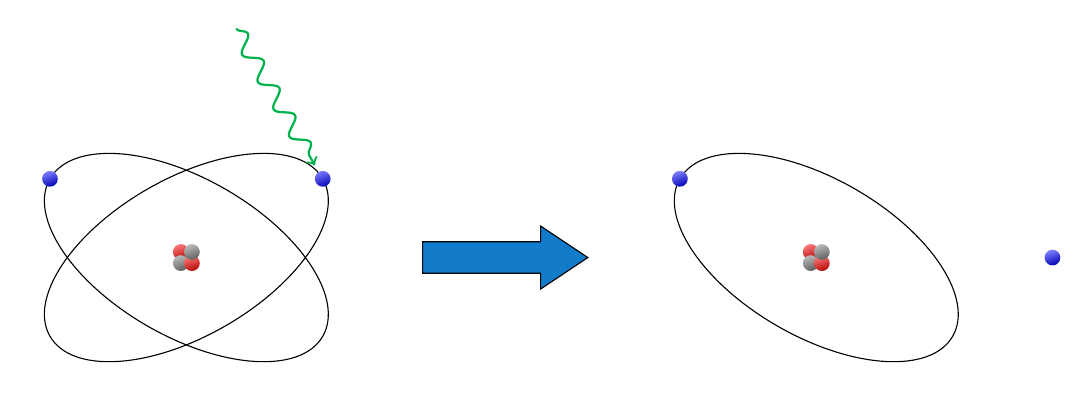
\begin{tikzpicture}
      %nucleo
      \shade[rotate=45,top color=red!50,bottom color=red!70!black,shading angle=20] (0,0.1) circle (0.1cm);
      \shade[rotate=45,top color=gray!50,bottom color=gray!70!black,shading angle=20] (-0.1,0) circle (0.1cm);
      \shade[rotate=45,top color=red!50,bottom color=red!70!black,shading angle=20] (0,-0.1) circle (0.1cm);
      \shade[rotate=45,top color=gray!50,bottom color=gray!70!black,shading angle=20] (0.1,0) circle (0.1cm);
      %orbite
      \draw[rotate=30] (0,0) ellipse (2cm and 1cm);
      \shade[rotate=30,top color=blue!50,bottom color=blue!70!black,shading angle=20] (2,0) circle (0.1cm);
      \draw[rotate=150] (0,0) ellipse (2cm and 1cm);
      \shade[rotate=150,top color=blue!50,bottom color=blue!70!black,shading angle=20] (2,0) circle (0.1cm);
      %fotone
      \draw[->,thick, teal!60!green, decorate, decoration={snake, segment length=4mm, amplitude=1mm,post length=1mm},rotate=30,rotate around={90:(2,0)}] (4.2,0) -- (2.2,0);
      %freccia
      \draw [fill=cyan!60!blue!,shift={(2.5 cm,0 cm)}] (0.5,0.2) -- (2,0.2) -- (2,0.4) -- (2.6,0) -- (2,-0.4) -- (2, - 0.2) -- (0.5,-0.2) -- cycle;
      \begin{scope}[shift={(8 cm,0 cm)}]
        %nucleo
        \shade[rotate=45,top color=red!50,bottom color=red!70!black,shading angle=20] (0,0.1) circle (0.1cm);
        \shade[rotate=45,top color=gray!50,bottom color=gray!70!black,shading angle=20] (-0.1,0) circle (0.1cm);
        \shade[rotate=45,top color=red!50,bottom color=red!70!black,shading angle=20] (0,-0.1) circle (0.1cm);
        \shade[rotate=45,top color=gray!50,bottom color=gray!70!black,shading angle=20] (0.1,0) circle (0.1cm);
        %orbite
        \draw[rotate=150] (0,0) ellipse (2cm and 1cm);
        \shade[rotate=150,top color=blue!50,bottom color=blue!70!black,shading angle=20] (2,0) circle (0.1cm);
        %elettrone
        \shade[top color=blue!50,bottom color=blue!70!black,shading angle=20] (3,0) circle (0.1cm);
      \end{scope}
    \end{tikzpicture}
\end{figure}

%L'idea alla base è quella di sfruttare il fatto che le particelle che attraversano un contenitore pieno di gas cedono energia e la possono cedere andando a produrre fenomeni di ionizzazione. Quindi sostanzialmente l'energia ricevuta da uno degli elettroni degli atomi che compongono il gas permette all'elettrone di essere espulso e quindi alla fine il risultato è la produzione di una coppia ione positivo-elettrone.
Il concetto di base è sfruttare il fatto che le particelle che attraversano un contenitore pieno di gas trasferiscono energia, che può essere utilizzata per produrre fenomeni di ionizzazione. In pratica, l'energia assorbita da uno degli elettroni degli atomi del gas può espellere l'elettrone, generando così una coppia composta da un ione positivo e un elettrone libero.

\begin{minipage}{0.395\textwidth}
   \begin{figure}[H]
      \centering
      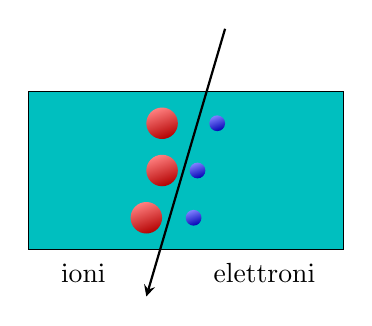
\begin{tikzpicture}
         %gas
         \draw[fill=teal!50!cyan!] (0,-1) -- (0,1) -- (4,1) -- (4,-1) -- cycle;
         \draw[-stealth,thick] (2.5,1.8) -- (1.5,-1.6);
         %particelle
         %prima fila
         \shade[top color=red!50,bottom color=red!70!black,shading angle=20] (1.7,0.6) circle (0.2cm);
         \shade[top color=blue!50,bottom color=blue!70!black,shading angle=20] (2.4,0.6) circle (0.1cm);
         %seconda fila
         \shade[top color=red!50,bottom color=red!70!black,shading angle=20] (1.7,0) circle (0.2cm);
         \shade[top color=blue!50,bottom color=blue!70!black,shading angle=20] (2.15,0) circle (0.1cm);
         %terza fila
         \shade[top color=red!50,bottom color=red!70!black,shading angle=20] (1.5,-0.6) circle (0.2cm);
         \shade[top color=blue!50,bottom color=blue!70!black,shading angle=20] (2.1,-0.6) circle (0.1cm);
         %nomi
         \node at (0.7,-1.3) {ioni};
         \node at (3,-1.3) {elettroni};
       \end{tikzpicture}
   \end{figure}
\end{minipage}
\begin{minipage}{0.6\textwidth}
   \vspace{0.5cm}Possiamo schematizzare un rivelatore al gas come un contenitore riempito di gas. Nel momento in cui passa una particella carica, questa particella produce coppie elettrone-ione, i quali hanno dimensioni e masse notevolmente differenti, fatto che comporta delle conseguenze soprattutto per quello che riguarda la raccolta del segnale. 
\end{minipage}

Chiaramente, nel momento in cui una particella attraversa un volume pieno di gas non viene prodotta una sola coppia: ne vengono prodotte un certo numero che dipende da quanta energia la particella deposita all'interno del gas.

Un tale sistema funziona come rivelatore perché abbiamo un segnale (che in questo caso è la produzione di coppie elettrone-ione) che indica il passaggio di una particella. Addirittura, se fossimo capaci di contare quante coppie sono state create potremmo avere un'informazione anche sull'energia che è stata depositata all'interno del rivelatore. 

Questi rivelatori a gas possono essere adoperati sia in current mode che in pulsed mode. La differenza sta nel fatto che in pulsed mode si produce un impulso elettrico ogni volta che passa una particella, mentre nella modalità current mode il flusso di particelle è così elevato che alla fine si produce una corrente continua il cui valore è proporzionale al flusso di particelle che sta incidendo sul rivelatore, dunque è come se si facesse una media di tanti impulsi che sono molto ravvicinati tra di loro in tempo, quindi non è più possibile distinguere un impulso dal successivo, ma si ha sostanzialmente una corrente continua.

\section{Ionizzazione}

\subsection{Meccanismi di ionizzazione}

I processi di interazione di una particella carica in un gas si dividono essenzialmente in due tipi di reazione:
\begin{enumerate}
   \item eccitazione;
   \item ionizzazione, in cui vengono creati un elettrone libero e uno ione.
\end{enumerate}
L'eccitazione di un atomo $X$ ad opera di una particella carica $p$ è
\begin{equation*}
   X + p \ce{->} X^* + p
\end{equation*}
ed è una reazione risonante, che richiede il trasferimento di un corretto valore di energia, in quato il valore di energia fornito deve corrispondere al salto energetico dell'elettrone.

Le sezioni d'urto tipiche nei gas nobili in risonanza sono dell'ordine di $\sigma \approx 10^{-17} \, \text{cm}^2$. Sebbene non vengano creati elettroni o ioni liberi, la molecola o l'atomo eccitati possono partecipare a ulteriori reazioni che portano all'ionizzazione.

%\comment{
\begin{approfondimento}[Le reazioni risonanti]
   \footnotesize
   Una "reazione risonante" è un concetto utilizzato in fisica, in particolare nel contesto delle reazioni nucleari e delle reazioni chimiche, per descrivere un fenomeno in cui la probabilità di una reazione aumenta notevolmente a causa della presenza di una "risonanza".
   
   Nel contesto delle reazioni nucleari, una reazione risonante si verifica quando l'energia dei nuclei che partecipano alla reazione corrisponde all'energia di uno stato eccitato (risonanza) del nucleo composto che si forma temporaneamente durante la reazione. Questo stato eccitato è di solito instabile e si disintegra rapidamente, ma la coincidenza tra l'energia dei reagenti e l'energia dello stato eccitato aumenta significativamente la probabilità che la reazione avvenga. In pratica, la sezione d'urto (una misura della probabilità di reazione) ha un picco molto alto a una specifica energia, corrispondente all'energia della risonanza. Questo fenomeno è comune nelle reazioni nucleari a basse energie, come quelle che avvengono nelle stelle o nei reattori nucleari.

   L'eccitazione è considerata una reazione risonante in alcuni contesti perché coinvolge un trasferimento di energia che coincide con l'energia specifica necessaria per portare un sistema (come un atomo o un nucleo) in uno stato eccitato, che è uno stato di energia superiore rispetto al suo stato fondamentale.

   I motivi per cui si parla di "risonanza" nel contesto dell'eccitazione sono i seguenti:
   \begin{enumerate}[leftmargin=0.5cm]
      \item Coincidenza Energetica: L'eccitazione avviene quando l'energia di una particella incidente (come un fotone o un elettrone) corrisponde esattamente all'energia di uno stato eccitato del sistema. Questa coincidenza energetica è una condizione di risonanza. Ad esempio, se un atomo assorbe un fotone la cui energia corrisponde alla differenza tra due livelli energetici dell'atomo, l'atomo può essere eccitato a uno stato superiore.
      \item Massima Probabilità di Assorbimento: Quando l'energia della particella incidente coincide con l'energia del livello eccitato, la probabilità che il sistema assorba l'energia e si ecciti è massima. Questo è analogo a ciò che accade nelle reazioni nucleari risonanti, dove la sezione d'urto raggiunge un picco a una certa energia.
      \item Effetto di Risonanza: La "risonanza" si riferisce alla condizione in cui un sistema risponde con un'amplificazione del segnale o dell'energia in ingresso quando quest'ultima corrisponde a una delle frequenze naturali del sistema. Nel caso dell'eccitazione, il sistema atomico o molecolare risponde fortemente (cioè si eccita) quando l'energia fornita è in risonanza con una delle sue frequenze naturali (o stati energetici quantizzati).
   \end{enumerate}
   In sintesi, l'eccitazione è una reazione risonante perché avviene più facilmente quando l'energia fornita corrisponde esattamente all'energia richiesta per raggiungere uno specifico stato eccitato del sistema, massimizzando così la probabilità di assorbimento e la conseguente eccitazione.
\end{approfondimento}
%}

Per una ionizzazione, che è
\begin{equation*}
   X + p \ce{->} X^+ + e^- + p
\end{equation*}
non esiste, naturalmente, un requisito energetico esatto e, in effetti, la sua sezione d'urto è leggermente superiore con $\sigma \approx 10^{-16} \, \text{cm}^2$. Tuttavia, il processo di ionizzazione avviene solamente se l'energia fornita supera una certa soglia, perché è necessario che l'elettrone venga strappato, quindi bisogna almeno fornire un'energia pari all'energia di prima ionizzazione del gas che stiamo adoperando.

Possiamo quindi dire che nella maggior parte dei casi avviene ionizzazione e ciò è probabilmente legato al fatto che l'energia per eccitare un elettrone non può assumere qualsiasi valore ma deve assumere dei valori ben precisi\footnote{Il Leo la pensa in maniera diametralmente opposta: dice che "La ionizzazione ha una soglia di energia relativamente alta e, poiché i trasferimenti di energia a basso valore sono più probabili, le reazioni di eccitazione generalmente prevalgono.", quindi non so a chi credere.}.

Gli elettroni e gli ioni creati dalla radiazione incidente stessa sono noti come ionizzazione primaria. In alcuni di questi casi di ionizzazione, tuttavia, viene trasferita una quantità di energia sufficientemente grande all'elettrone (raggi delta), tale che questo elettrone crea a sua volta coppie ione-elettrone. Quest'ultima ionizzazione è nota come ionizzazione secondaria. Se la loro energia è sufficientemente alta, gli elettroni di ionizzazione secondaria possono anche ionizzare ulteriormente, e così via fino a raggiungere la soglia per le reazioni di ionizzazione.

\comment{Se guardiamo i meccanismi di interazione delle particelle in un gas, scopriamo in realtà non sono possibili soltanto processi di ionizzazione degli atomi e delle molecole che compongono il gas, ma è possibile anche che si verifichi un fenomeno di eccitazione. Quindi andando a guardare alle tipologie di interazioni che possono avvenire, possiamo avere o che la particella X cede una porzione della sua energia che è in grado di eccitare l'elettrone e quindi portarlo a un livello eccitato (e oppure è possibile, come abbiamo detto prima, andare a ionizzare la molecola o l'atomo del gas e quindi produrre una coppia $\text{X}^+ - e^+$. Questo . In termini di sezione d'urto possiamo dire che i processi di ionizzazione sono processi più frequenti, più probabili, perché abbiamo una sezione d'urto dell'ordine di $10^{-16}\; \rm cm^2$, in confronto ai processi di eccitazione che hanno una sezione d'urto dell'ordine di $10^{-17}\; \rm cm^2$.  Quindi, a seguito del processo di ionizzazione si producono delle particelle, in particolare elettroni e ioni, che a loro volta in determinate condizioni potrebbero innurre e nascare dei fenomeni di ionizzazioni secondarie. Quindi abbiamo sia dei prodotti diretti di prima ionizzazione sia eventualmente dei prodotti secondari. Ora vedremo in che condizioni si innescano questi processi secondari.}

\subsection{W-values}
Ci chiediamo adesso quante coppie di ioni ed elettroni si formano. Siamo particolarmente interessati a questa informazione perché il numero di coppie ci potrebbe dare un'informazione sull'energia depositata.

Ingenuamente potremmo pensare che il numero medio di coppie che si formano siano date dal rapporto tra l'energia depositata e il potenziale di prima ionizzazione di un gas, il quale normalmente assume dei valori che dipendono dal tipo di gas che stiamo adoperando e che assume valori compresi tra i 10 e i 25 eV. Ciò sarebbe corretto se avvenissero soltanto ionizzazioni, ma nella realtà avviene anche l'eccitazione, per cui nel valutare il numero di coppie ione-elettrone che si formano dobbiamo tenere conto del fatto che parte dell'energia che viene depositata viene utilizzata per eccitare gli elettroni, quindi non viene totalmente adoperata per ionizzazione per creare coppie. Ecco perché l'energia media per creare una coppia ione-elettrone è un po' più alta rispetto al potenziale di prima ionizzazione, variando normalmente tra i 25 e i 40 eV.

\begin{figure}[H]
   \centering
   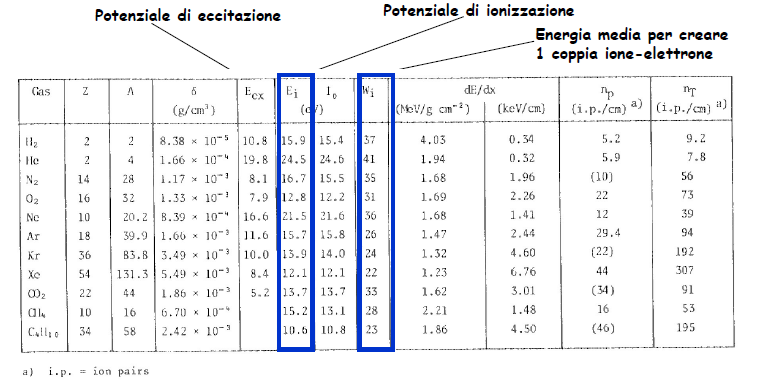
\includegraphics[width=\textwidth]{immagini/potenziali_ionizzazione.png}
\end{figure}

In questa tabella possiamo vedere, per diverse tipologie di gas, i valori del potenziale di eccitazione e di prima ionizzazione, indicate rispettivamente con $E_{\rm ex}$ e $E_{\rm i}$, e l'energia media per creare una coppia ione-elettrone, indicata con $W$. Notiamo che per eccitare gli atomi sono necessarie energie dell'ordine della decina di eV, mentre per ionizzare il potenziale di prima ionizzazione assume valori un po' più alti, tra i 10 e i 20 eV. Se invece consideriamo l'energia media per creare una coppia ione-elettrone, questo risulta essere un po' più grande rispetto al potenziale di prima ionizzazione, in quanto tiene conto dei fenomeni di eccitazione. Se ad esempio utilizzassimo dell'idrogeno $\rm H_2$, l'energia media per creare una coppia è pari a 37 eV.

\vspace{0.4cm}

\begin{minipage}{0.245\textwidth}
   \begin{center}
      \begin{tabular}{|c|c|}
         \hline
         &\\[-0.4cm]
         Gas & $W$ (eV)\\[0.1mm]
         &\\[-0.4cm]
         \hline
         &\\[-0.4cm]
         Ne & $36.3$\\[0.1mm]
         \hline
         &\\[-0.4cm]
         Ar & $26.2$\\[0.1mm]
         \hline
         &\\[-0.4cm]
         Xe & $21.5$\\[0.1mm]
         \hline
         &\\[-0.4cm]
         $\rm P10$ & $26$\\[0.1mm]
         \hline
      \end{tabular}
   \end{center}
\end{minipage}
\begin{minipage}{0.75\textwidth}
   L'energia media per creare una coppia $W$ è quella che ci permette di stimare quante coppie elettrone-ione si formano all'interno di un gas. Il valore di $W$ dipende dal tipo di gas, ad esempio nella tabella a fianco possiamo vedere i valori per dei gas nobili, in quanto spesso nei rivelatori a gas si utilizzano gas nobili, ma si utilizzano tante volte anche delle miscele come il $\rm P10$, che è una composizione di argon al 90\% e di metano ($\rm CH_4$) al 10\%.
\end{minipage}

\vspace{0.4cm}

In realtà il valore di $W$ dipende leggermente anche dal tipo di particella e dall'energia. Ad esempio nel seguente grafico vediamo dei valori di $W$ per diverse particelle incidenti in funzione dell'energia

\begin{figure}[H]
   \centering
   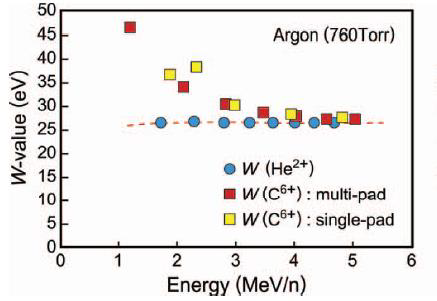
\includegraphics[width=0.6\textwidth]{immagini/vallori_W_energia.png}
\end{figure}

Vediamo che c'è una leggerissima dipendenza dall'energia e dal tipo di particella, quindi non è sufficiente conoscere solamente il gas, ma in realtà purtroppo questo valore può dipendere leggermente anche dalla particella.

In particolare, per valutare il valore del potenziale medio per creare la coppia se si adopera una miscela di gas si utilizza una sorta di media pesata, un po' come abbiamo visto nel caso della perdita di energia nei composti.

\begin{approfondimento}[W-values per miscele e numero di coppie]
   \footnotesize
   Metto questo approfondimento perché la professoressa non spiega esplicitamente come calcolarlo. Come al solito ringraziamo chatgpt.\\
   Se abbiamo una miscela di gas, il $W$-value della miscela può essere calcolato in base ai $W$-value dei singoli componenti della miscela e alle loro frazioni molari o volumetriche. L'espressione generale è data da
   \begin{equation*}
      W_{\text{mix}} = \frac{1}{\sum_i \frac{x_i}{W_i}}
   \end{equation*}
   dove $W_{\text{mix}}$ è il $W$-value della miscela di gas e $x_i$ e $W_i$ sono rispettivamente la frazione molare o volumetrica e il $W$-value del componente $i$-esimo nella miscela.\\
   \comment{Se ad esempio abbiamo una miscela composta da due gas, A e B, con frazioni volumetriche $x_A$ e $x_B$ rispettivamente, e $W$-value $W_A$ e $W_B$, il $W$-value della miscela sarebbe:
   \begin{equation*}
      W_{\text{mix}} = \frac{1}{\frac{x_{\rm A}}{W_{\rm A}} + \frac{x_{\rm B}}{W_{\rm B}}}
   \end{equation*}
   Questo calcolo può essere esteso a miscele con più di due componenti, semplicemente aggiungendo più termini nella somma.\\}
   \E da notare che il $W$-value dipende dalle proprietà fisiche del gas e dalle condizioni operative, come la pressione e la temperatura. Tuttavia, in prima approssimazione, la formula sopra riportata è utile per calcolare il valore $W$ di una miscela a condizioni standard.\\[0.2cm]
   \textbf{$\boldsymbol{W}$-per unità di percorso}\\
   Il $W$-value si può esprimere anche in termini di unità di percorso (ad esempio, per calcolare l'energia media necessaria per creare una coppia di ioni per unità di lunghezza percorsa da una particella carica in un gas). Per fare ciò, si può utilizzare una relazione che coinvolge la perdita di energia per unità di lunghezza, cioè il $\dv*{E}{x}$. In particolare, la relazione tra il $W$-value in unità di percorso e la perdita di energia per unità di lunghezza $\dv*{E}{x}$ è data da
   \begin{equation*}
      W_{\text{path, mix}}
      =\frac{\sum_i x_i \cdot \qty( \dv{E}{x} )_i}{\sum_i x_i \cdot \frac{1}{W_i}}
   \end{equation*}
   dove $(\dv*{E}{x})_i$ è la perdita di energia per unità di lunghezza del componente $i$-esimo in eV/cm.\\
   \E da notare che l'espressione per il calcolo del $W$-value della miscela è una media armonica ponderata dei $W$-value dei singoli componenti della miscela. In generale, una media armonica ponderata è utilizzata quando si vuole combinare quantità che sono inversamente proporzionali al valore di interesse. In questo caso il significato fisico di questa media armonica ponderata è che in una miscela di gas, il $W$-value della miscela sarà dominato dai componenti con i $W$-value più bassi, ovvero quelli per cui è necessaria meno energia per produrre una coppia di ioni. Il contributo di ciascun componente al $W$-value complessivo è proporzionale alla sua frazione molare o volumetrica.\\[0.2cm]
   \textbf{Coppie create per unità di percorso}\\
   Il numero di coppie prodotte per unità di lunghezza è in generale dato da
   \begin{equation*}
      n_{\rm coppie}=\frac{\dv{E}{x}}{W}
   \end{equation*}
   Nel caso di una miscela, il numero di coppie di ioni prodotte per unità di lunghezza può essere espresso come:
   \begin{equation*}
      n_{\rm coppie}
      =\sum_i \frac{x_i \cdot \qty( \dv{E}{x} )_i}{W_i}
   \end{equation*}
\end{approfondimento}

Facciamo un esempio numerico: immaginiamo di avere una miscela composta da argon all'80\% e da anidride carbonica $\rm CO_2$ al 20\%. Se voglio sapere quanti coppie al centimetro si formano, dobbiamo conoscere sia i valori dei potenziali $W$ che quelli della perdita di energia per unità di percorso di entrambi i gas. Controllando i valori tabulati si ha che
\begin{equation*}
   n_{\rm coppie}
   =\frac{\qty(\dv{E}{x})_{\rm Ar}}{W_{\rm Ar}} \cdot \%_{\rm Ar} + \frac{\qty(\dv{E}{x})_{\rm CO_2}}{W_{\rm CO_2}} \cdot \%_{\rm CO_2}
   =\frac{2440}{26} \cdot 0.8 + \frac{3010}{33} \cdot 0.2
   =93 \; \rm \frac{coppie}{cm}
\end{equation*}
\subsection{Fluttuazioni e risoluzione}

Assumendo che il $W$-value del gas sia costante per un dato tipo di radiazione, l'energia depositata sarà proporzionale al numero $N$ di coppie ione-elettrone formate e può essere determinata se viene effettuata una misurazione corrispondente del numero di coppie di ioni, in quanto tale numero è dato dal rapporto tra l'energia depositata e il $W$-value.

Oltre al numero medio di coppie di ioni formate da ciascuna particella incidente, è di interesse anche la fluttuazione nel loro numero per particelle incidenti di identica energia. Queste fluttuazioni stabiliranno un limite fondamentale sulla risoluzione energetica che può essere raggiunta in qualsiasi rivelatore basato sulla raccolta degli ioni. Possiamo supporre, in prima approssimazione, che la formazione di ogni coppia di ioni sarà considerata un processo di Poisson, nel senso che il numero totale di coppie di ioni formate segue la distribuzione di Poisson ed è quindi soggetto a fluttuazioni statistiche caratterizzate da una deviazione standard pari alla radice quadrata del numero medio di coppie formatisi. Nella tabella seguente possiamo vedere degli esempi di fluttuazioni del numero di particelle nel caso di un gas avente $W=30 \rm \; eV$ al variare dell'energia depositata dalle particelle incidenti:

\begin{center}
   \begin{tabular}{llll}
      Energia depositata & n° coppie & $\sqrt{N}$ & $\sqrt{N}/N$\\[0.2cm]
      100 keV & 3330 & 58 & 1.7\%\\[0.2cm]
      1 MeV & 33300 & 183 & 0.5\%
   \end{tabular}
\end{center}

Notiamo che la risoluzione, dal momento che l'energia è proporzionale al numero di coppie, può essere espressa in termini del rapporto $\sqrt{N}/N$. Da ciò segue che più è grande il numero di coppie $N$, più la risoluzione dovrebbe essere migliore.

Come discusso nel capitolo \ref{chap:caratteristiche_rivelatori}, molti rivelatori di radiazioni mostrano una fluttuazione intrinseca inferiore a quella prevista da questo modello semplificato. Per sistemare tale incongruenza si introduce il fattore di Fano $F$ come una costante empirica per cui la varianza prevista deve essere moltiplicata per ottenere la varianza osservata sperimentalmente:
\begin{equation*}
   F=\frac{\text{varianza osserivata in $N$}}{\text{varianza prevista da Poisson $(=N)$}}
\end{equation*}
Il fattore di Fano rappresenta in un certo senso la frazione di tutta l'energia della particella incidente che viene convertita in portatori di informazione all'interno del rivelatore (cioè gli ioni). Se l'intera energia della radiazione incidente fosse sempre convertita in coppie di ioni, il numero di coppie prodotte sarebbe sempre esattamente lo stesso e non ci sarebbe alcuna fluttuazione statistica. In queste condizioni, il fattore di Fano sarebbe zero. Tuttavia, se solo una piccola frazione della radiazione incidente è convertita, le coppie di ioni si formerebbero a grande distanza l'una dall'altra e con una probabilità relativamente bassa, e ci sarebbe un buon motivo per aspettarsi che la distribuzione nel loro numero segua una distribuzione di Poisson. Nei gas, il fattore di Fano è osservato empiricamente essere inferiore a 1, quindi le fluttuazioni sono minori di quanto previsto basandosi esclusivamente sulle statistiche di Poisson. Segue immediatamente che minore è $F$ migliore è la risoluzione. Chiaramente, nel caso in cui gli eventi seguano la distribuzione di Poisson $F=1$ e la risoluzione dipenderà soltanto dal numero di particelle in maniera inversamente proporzionale.

Alla luce di ciò, per un rivelatore a gas la risoluzione energetica può essere espressa come\footnote{Nelle slide la professoressa definisce la risoluzione per i rivelatori a gas come
\begin{equation*}
   R
   =2.35\frac{\sigma_E}{E}
   =2.35\frac{W\sqrt{FN}}{WN}
   =2,35 \cdot \sqrt{\frac{F}{N}}
\end{equation*}
Non ho capito quanto sia lecita l'assunzione $\sigma_E=W\sigma_N$, ma la riporto per completezza.}
\begin{equation*}
   R
   =2,35 \cdot \sqrt{\frac{FW}{E}}
   =2,35 \cdot \sqrt{\frac{FW}{WN}}
   =2,35 \cdot \sqrt{\frac{F}{N}}
\end{equation*}

\section{Fenomeni di trasporto nei gas}

Per i rivelatori a gas, è estremamente importante comprendere il moto degli elettroni e degli ioni nel gas, in quanto esso influenza diverse caratteristiche operative del rivelatore. Infatti, una volta create queste coppie, dobbiamo essere in grado di raccoglierle in qualche modo e tradurle in un segnale elettrico. Vediamo allora i diversi meccanismi che possono subire tali particelle cariche all'interno di un gas.

\subsection{Diffusione}

In assenza di un campo elettrico, gli elettroni e gli ioni prodotti dalla radiazione che attraversa il gas si diffondono uniformemente verso l'esterno dal loro punto di creazione. Nel processo, subiscono molteplici collisioni con le molecole di gas e perdono la loro energia, raggiungendo in questo modo rapidamente l'equilibrio termico con il gas. Il libero cammino medio, cioè la distanza media percorsa dopo la quale si ha un'interazione, varia tra i $10^{-8}$ m e i $10^{-6}$ m.\footnote{In particolare il Knoll dice che "Gli atomi o le molecole neutre del gas sono in costante moto termico, caratterizzato da un libero cammino medio che per i gas in condizioni standard è tipicamente di circa $10^{-6} - 10^{-8}$ m. Gli ioni positivi o gli elettroni liberi creati all'interno del gas partecipano anch'essi al moto termico casuale e quindi tendono a diffondersi dalle regioni ad alta densità."}

A energie termiche\footnote{Si intende che l'energia delle particelle è esclusivamente dovuta all'agitazione termica causata dalla temperatura del sistema.}, le velocità delle cariche sono descritte dalla distribuzione di Maxwell - Boltzmann, che fornisce una velocità media 
\begin{equation*}
   v \propto \sqrt{\frac{k_B T}{m}}
\end{equation*}
dove $k_B$ è la costante di Boltzmann, $T$ è la temperatura e $m$ è la massa della particella. A causa di tale dipendenza, poiché la massa degli elettroni è molto più piccola di quella degli ioni segue che gli elettroni diffondono con velocità molto più elevate rispetto a quelle degli elettroni, cioè $v_{\rm elettroni} \gg v_{\rm ioni}$. In particolare, a temperatura ambiente, quindi circa $22 \rm \; ^{\circ}C$, si ha che $v_{\rm elettroni} \sim 10^6 \; \rm cm/s$ e $v_{\rm ioni} \sim 10^4 \; \rm cm/s$.

Secondo la teoria cinetica, si può dimostrare che la distribuzione lineare (cioè delle distanze percorse) delle cariche dopo un tempo di diffusione $t$ ha un andamento di tipo gaussiano con centroide in $x=0$:
\begin{equation*}
   \dv{N}{x}=\frac{N_0}{\sqrt{4\pi D t}} \exp\left(-\frac{x^2}{4Dt}\right)
\end{equation*}
dove $N_0$ è il numero totale di cariche, $x$ la distanza dal punto di creazione e $D$ il coefficiente di diffusione. La deviazione standard in $x$ è quindi
\begin{equation*}
   \sigma(x) = \sqrt{2Dt}
\end{equation*}
Questo ragionamento è stato fatto nel caso unidimensionale, ma nella realtà dobbiamo considerare il caso tridimensionale, perché le particelle si possono diffondere in tutte le direzioni dello spazio. Se si considerano tre dimensioni, la dispersione sferica è data da
\begin{equation*}
   \sigma(r)=\sqrt{6Dt}
\end{equation*}
dove $r$ è la distanza radiale. Ad esempio, la dispersione radiale degli ioni nell'aria in condizioni normali è di circa 1 mm dopo 1 secondo.

Il coefficiente di diffusione è un parametro che può essere calcolato dalla teoria cinetica e si può dimostrare che vale
\begin{equation*}
   D=\frac{1}{3} \lambda v
\end{equation*}
dove $\lambda$ è il libero cammino medio dell'elettrone o dello ione nel gas. Per un gas ideale classico, il libero cammino medio è correlato alla temperatura $T$ e alla pressione $p$ da
\begin{equation*}
   \lambda=\frac{1}{\sqrt{2}} \frac{kT}{\sigma_0 p}
\end{equation*}
dove $\sigma_0$ è la sezione d'urto totale per una collisione con una molecola di gas. Sostituendo le espressioni di $v$ e $\lambda$ si ottiene l'espressione esplicita
\begin{equation*}
   D=\frac{2}{3\sqrt{\pi}} \frac{1}{p\sigma_0} \sqrt{\frac{(kT)^3}{m}}
\end{equation*}
Da cui si evince la dipendenza di $D$ dai vari parametri del gas (temperatura e pressione), dalla massa della particella e dalla sezione d'urto di interazione.

\subsection{Ricombinazione}
Può succedere che, durante il moto di diffusione, ad un certo punto avvengano collisioni tra ioni positivi ed elettroni liberi\footnote{Il Leo dice: "In assenza di campo elettrico, le coppie elettrone-ione tenderanno a ricombinarsi sotto la forza della loro attrazione elettrica". Credo che questa sia un'interpretazione più corretta, visto che sono i campi ad interagire, o mi sbaglio?}, le quali danno luogo ad una ricombinazione in cui l'elettrone è catturato dallo ione, riportando così l'atomo ad una condizione di neutralità in termini di cariche. In tale processo si ha inoltre l'emissione di un fotone:
\begin{equation*}
   e^- + X^+ \ce{->} X + h\nu
\end{equation*}
In alternativa, uno ione positivo potrebbe subire una collisione con uno ione negativo nella quale l'elettrone in più dell'anione è trasferito sul catione, neutralizzando così entrambi. Anche in questo caso si avrà la produzione di un fotone
\begin{equation*}
   X^+ + Y^- \ce{->} XY + h\nu
\end{equation*}

\begin{approfondimento}[L'electron attachment]
   \footnotesize Per capire come possa avvenire questa seconda reazione, è necessario introdurre un altro fenomeno che avviene all'interno dei gas, ossia l'electron attachment.\\
   Tale fenomeno riguarda la cattura degli elettroni liberi ad opera di atomi elettronegativi formando così ioni negativi, i quali sono molto simili agli ioni positivi del gas formatisi nel processo di ionizzazione, ma questi avranno carica opposta:
   \begin{equation*}
      e^- + X \ce{->} X^- + h\nu
   \end{equation*}
   Gli atomi elettronegativi sono atomi che hanno la shell esterna quasi piena, per cui l'aggiunta di un ulteriore elettroni risulta in una cessione di energia, di conseguenza lo ione negativo che si forma è stabile. L'energia rilasciata in questa cattura è conosciuta come affinità elettronica, ed è un indicatore della tendenza degli atomi neutri del gas a formare ioni negativi.% L'ossigeno costituisce un esempio di gas che cattura velocemente gli elettroni diffusi.
   \\Per maggiori informazioni si veda \textit{S. Arena, V. Favitta,"Chimica Nino"}.
\end{approfondimento}

\E chiaro che, se vogliamo rivelare il passaggio della particella, questi processi di ricombinazione devono essere assolutamente evitati, in quanto la rivelazione si basa sulla misura delle cariche che sono state prodotte: se le cariche scompaiono a seguito della ricombinazione, l'informazione viene persa.

Bisogna quindi assicurarsi che le cariche sopravvivano nel rivelatore per un tempo sufficiente a effettuare la raccolta delle cariche e quindi a formare un segnale elettrico. Di conseguenza è necessario agire dall'esterno, perché altrimenti le cariche prima o poi si ricombineranno, e ciò avverrà in tempi abbastanza brevi (ad esempio, nel caso di una miscela di ossigeno in 140 ns le ricombinazioni si sono quasi del tutto esaurite, quindi le cariche prodotte a seguito della ionizzazione sono praticamente ormai perse, cioè non si possono utilizzare per produrre un segnale elettrico). 

\subsection{Migrazione}
Per cercare di raccogliere le cariche, bisogna farle migrare. Per fare ciò si deve applicare un campo elettrico, dunque una forza che in linea di principio dovrebbe far accelerare queste particelle all'interno del gas. In realtà le particelle non arrivano a seguire un moto accelerato perché interagiscono continuamente con le molecole presenti nel gas, tuttavia riescono ad avere un moto di migrazione verso gli elettrodi utilizzati per generare il campo elettrico e questa migrazione avviene con una velocità che chiamiamo \textit{velocità di deriva o di drift}. Questa velocità di deriva si sovrappone al moto casuale dovuto all'agitazione termica e dipende dalle caratteristiche del campo elettrico applicato. In particolare si può dimostrare che essa si può esprimere come
\begin{equation*}
   v_{\rm drift}=\mu\frac{E}{p}
\end{equation*}
dove $\mu$ è un fattore che prende il nome di mobilità e il rapporto tra il campo elettrico e la pressione del gas considerato è il cosiddetto campo elettrico ridotto.

Risulta evidente che applicare un campo elettrico maggiore comporta una velocità di drift maggiore, ma anche la pressione avrà la sua importanza, in quanto aumentare la pressione del gas vuol dire sostanzialmente aumentare la densità di atomi presenti all'interno del gas e dunque la possibilità di avere urti. Ne segue che l'aumentare della pressione riduce la velocità di drift.

Sebbene considereremo la mobilità come se fosse un fattore costante, precisiamo che in realtà essa dipende dal tipo di particella che si considera e dall'energia in gioco, come mostrato dal seguente grafico, in cui è riportato l'andamento della velocità di drift in funzione di $E/p$:
\begin{figure}[H]
   \centering
   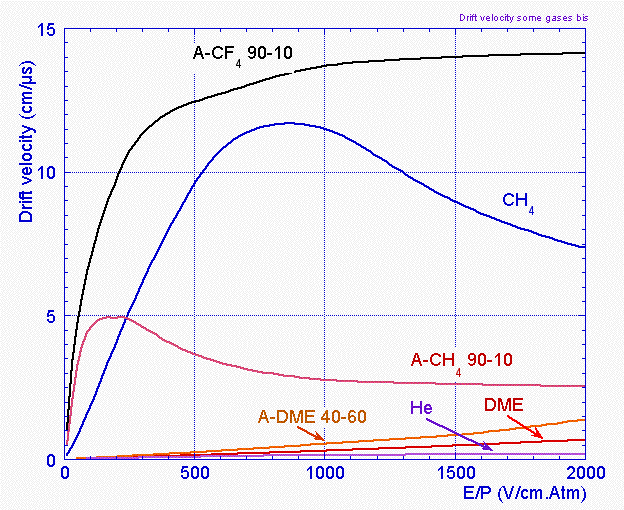
\includegraphics[width=0.6\textwidth]{immagini/mobilita.png}
\end{figure}
Se $\mu$ fosse esattamente costante dovremmo osservare delle rette, ma in pratica osserviamo tale andamento solo per bassi valori di campo elettrico. Tuttavia, dato che le condizioni in cui lavoriamo con i rivelatori a gas ricadono proprio in tale regione, possiamo tranquillamente supporre che la mobilità assuma un valore costante. Essa si esprime in $\rm m^2 \, atm \, V^{-1} \, s^{-1}$ e in generale assume valori molto più alti per gli elettroni piuttosto che per gli ioni, e ciò è legato alle masse in gioco. Ad esempio, in un gas come l'argon la mobilità degli elettroni è pari a $\mu_{\rm e}=2 \cdot 10^4$ mentre quella degli ioni è pari a $\mu_{\rm ioni}=1,5$. In conseguenza a queste profonde differenze nei valori di mobilità, quando si verifica una migrazione a seguito di un campo elettrico ci aspettiamo che gli elettroni si muovano molto velocemente mentre gli ioni abbiano una migrazione molto più lenta. Sempre in corrispondenza dell'argon, abbiamo che in esso $v_{\rm e}=3 \cdot 10^5 \; \rm cm/s$ e $v_{\rm ioni}=3 \cdot 10^2 \; \rm cm/s$, cioè differiscono di un fattore $10^3$. Nella seguente tabella possiamo vedere altri valori per altre miscele che confermano grossomodo questo fattore di differenza tra le due categorie di particelle:
\begin{center}
   \begin{tabular}{|c|c|c|}
     \hline
     &&\\[-0.4cm]
     Gas & $v_{\rm elettroni}$ (cm/s) & $v_{\rm ioni}$ (cm/s)\\
     \hline
     &&\\[-0.35cm]
     Ar & $3 \cdot 10^5$ & $3 \cdot 10^2$\\
     \hline
     &&\\[-0.35cm]
     He & $4 \cdot 10^5$ & $2 \cdot 10^3$\\
     \hline
     &&\\[-0.35cm]
     Ne & $10^6$ & $9 \cdot 10^2$\\
     \hline
     &&\\[-0.35cm]
     $\rm N_2$ & $4 \cdot 10^5$ & $5 \cdot 10^2$\\
     \hline
     &&\\[-0.35cm]
     $\rm H_2$ & $7 \cdot 10^5$ & $3 \cdot 10^3$\\
     \hline
     &&\\[-0.35cm]
     $\rm 95\% A + 5\% CO_2$ & $3.5 \cdot 10^6$ & $-$\\
     \hline
     &&\\[-0.35cm]
     $\rm CO_2$ & $10^5$ & $-$\\
     \hline
     &&\\[-0.35cm]
     $\rm CH_4$ & $1.5 \cdot 10^6$ & $-$\\
     \hline
   \end{tabular}
\end{center}
La conseguenza principale di questa enorme differenza nelle velocità tra ioni ed elettroni è che se volessimo raccogliere tutte le cariche prodotte dovremmo aspettare tempi elevati. Infatti gli elettroni dovranno arrivare fino all'anodo mentre gli ioni positivi fino al catodo\footnote{A patto di apparire prolissi, specifichiamo che per gli ioni positivi la velocità di drift è diretta come il campo elettrico, cioè dall'anodo (positivo) verso il catodo (negativo), mentre per gli elettroni ha direzione opposta.}, quindi devono percorrere uno spazio pari più o meno delle dimensioni del rivelatore stesso, e se consideriamo rivelatori della decina di centimetri possiamo stimare che per raccogliere le cariche dovute agli elettroni sono necessari tempi abbastanza brevi, dell'ordine dei microsecondi, mentre per raccogliere anche le cariche dovute agli elettroni dovremmo aspettare tempi molto più lunghi, dell'ordine dei millisecondi.

\newpage

\section{Struttura base di un rivelatore a gas}
Lo schema di principio di un rivelatore a gas include un recipiente a tenuta di gas con all'interno due
elettrodi per generare un campo elettrico e quindi una differenza di potenziale tra questi.

Un primo esempio di elettrodi che si possono adoperare è quello in cui essi sono piani e paralleli, come se costituissero un condensatore piano:

\begin{figure}[H]
   \centering
   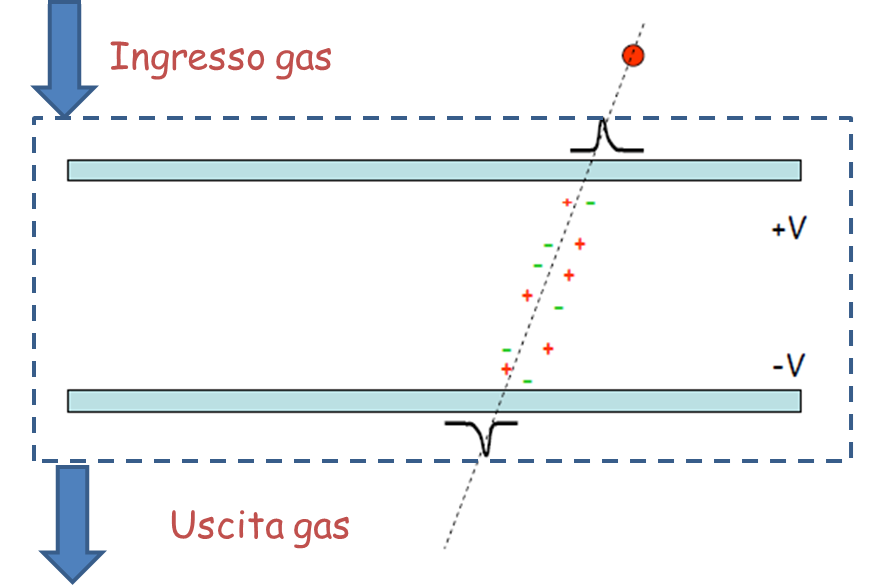
\includegraphics[width=0.6\textwidth]{immagini/modello_riv_gas_condensatore.png}
\end{figure}

Come vediamo in figura, al passaggio di una carica si genera ionizzazione e i prodotti della ionizzazione che sono gli elettroni e gli ioni incominciano a migrare a seguito dell'effetto del campo elettrico creato dagli elettrodi.

Per quanto riguarda le caratteristiche del gas, esso si può trovare o in condizioni statiche, quindi viene inserito nella camera e sigillato, oppure in condizioni dinamiche, per cui si hanno dei flussi continui in quanto i rivelatori possiedono un ingresso e un'uscita del gas in maniera tale avere sempre un ricircolo e avere una miscela di gas sempre corrispondente alle percentuali che sono state fissate all'inizio. Quest'ultimo è il regime in cui lavorano soprattutto i rivelatori che non hanno una tenuta ottimale.

%\subsection{Misura del segnale}
\subsection{Formazione dell'impulso}
In generale possiamo schematizzare un rivelatore gas come un condensatore, il quale viene polarizzato\footnote{Polarizzare un condensatore significa applicare una tensione ai suoi terminali in modo da stabilire una differenza di potenziale tra le sue armature. In particolare, si parla di polarizzazione quando il condensatore è polarizzato, cioè ha un lato che deve essere collegato al polo positivo e un lato che deve essere collegato al polo negativo dell'alimentazione.} attraverso una resistenza $R$ di valore molto elevato ($10^7-10^8 \; \Omega$).

\vspace{-0.1cm}

\begin{minipage}{0.395\textwidth}
   \begin{figure}[H]
      \centering
      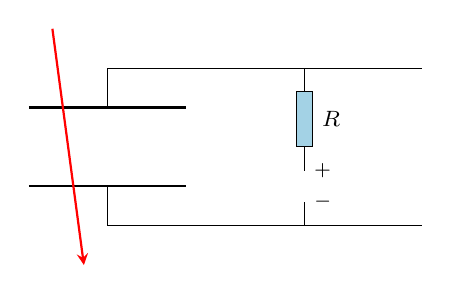
\begin{tikzpicture}
         %condensatore
         \draw[thick] (-1,0.5) -- (1,0.5);
         \draw[thick] (-1,-0.5) -- (1,-0.5);
         \draw (0,0.5) -- (0,1) -- (4,1);
         \draw (0,-0.5) -- (0,-1) -- (4,-1);
         %resistenza
         \draw (2.5,1) -- (2.5,-0.3) node[right] {\scriptsize$+$};
         \draw (2.5,-0.7) node[right] {\scriptsize$-$} -- (2.5,-1);
         \draw[fill=cyan!60!gray!50!] (2.4,0.7) -- (2.6,0.7) -- (2.6,0) node[midway, right] {\footnotesize$R$} -- (2.4,0) -- cycle;
         %segnale
         \draw[red,thick, -stealth] (-0.7,1.5) -- (-0.3,-1.5);
       \end{tikzpicture}
   \end{figure}
\end{minipage}
\begin{minipage}{0.6\textwidth}
   \vspace{0.5cm}Il motivo è che quando le cariche si avvicinano agli elettrodi (gli elettroni vanno verso l'anodo, gli ioni positivi verso il catodo), sugli elettrodi si genera una leggera variazione della tensione, proprio per il fatto che sono arrivate queste cariche, le quali quindi inducono una variazione nel valore di potenziale presente sugli elettrodi.
\end{minipage}

\vspace{0.1cm}

Se quindi gli elettrodi non fossero polarizzati, sarebbero destinati a scaricarsi velocemente. Dal momento che però gli elettrodi sono mantenuti a una differenza di potenziale costante attraverso un generatore di tensione, quello che succede è che la tensione viene subito riportata al valore nominale.

\begin{esempio}
   Come abbiamo detto, nel momento in cui passa una particella si producono delle cariche che producono una leggera variazione di tensione in queste piastre, ma grazie al collegamento con il generatore di tensione il potenziale viene immediatamente riportato al valore nominale. La velocità con cui ciò avviene dipende dalla resistenza del circuito, in quanto abbiamo sostanzialmente un circuito $RC$ e quindi la velocità del processo è stabilita dalla legge di carica di un condensatore nel caso in cui la carica iniziale non è nulla:
   \begin{equation*}
      V(t)=V_0 - (V_0 - \Delta V) e^{-\frac{t}{\tau}}
   \end{equation*}
   dove comanda il fattore $\tau=RC$, quindi più è grande $R$ più lenta sarà la risalita verso il valore nominale.\\
   Cerchiamo ora di capire quanto varia questa tensione tramite un esempio numerico. Supponiamo che gli elettrodi si trovino ad una differenza di potenziale $V_0=500 \; \rm V$ e che costituiscano un condensatore di capacità $C=50 \; \rm pF$. Immaginiamo poi che passi una particella di energia $5 \; \rm MeV$ che riesce a depositare tutta la sua energia all'interno del condensatore, quindi $E_{\rm dep}=5 \; \rm MeV$ e andiamo a valutare quanto vale la differenza di potenziale che si genera ai capi del condensatore a seguito della produzione di carica per ionizzazione.\\
   Innanzitutto calcoliamo la carica viene prodotta e che viene raccolta da ciascun elettrodo. Per fare ciò basta calcolare il numero di coppie prodotte e moltiplicare queste per la carica dell'elettrone:
   \begin{equation*}
      Q=e\frac{E_{\rm dep}}{W}
   \end{equation*}
   Se adesso dividiamo questa carica per la capacità del condensatore otteniamo la differenza di potenziale che si genera a seguito dell'interazione: supponendo per semplicità $W=1$, avremo
   \begin{equation*}
      \Delta V
      =\frac{Q}{C}
      =e\frac{E_{\rm dep}}{WC}
      =0.5 \; \rm mV
   \end{equation*}
   Quello che quindi succede è che a seguito del passaggio di una particella si produce un segnale elettrico e di conseguenza una variazione del valore di tensione, che abbiamo trovato essere dell'ordine di mezzo mV. Capiamo quindi che sono segnali veramente piccoli da rivelare, per cui bisogna cercare di rallentare il più possibile la risalita verso il valore nominale di tensione. Ecco spiegato perché si adoperano valori di resistenze elevati.
\end{esempio}

%\vfill

%\subsection{Formazione dell'impulso}

Quando le cariche prodotte vengono raccolte, la tensione agli elettrodi diminuisce dal valore $V_0$ al valore $V_0 - ne/C$, per poi ritornare al valore $V_0$ con legge di carica
esponenziale avente velocità dipendente dalla costante di tempo $RC$.\footnote{Nelle slide la professoressa riporta questo grafico smussato. A livello teorico è giusto che ci sia un punto angoloso, ma come dice il Knoll: "In qualsiasi situazione reale, la radiazione incidente crea coppie di ioni su una gamma di posizioni all'interno della camera. Le discontinuità nette mostrate risultano quindi in qualche modo 'sfumate' nella forma dell'impulso risultante."}

\begin{figure}[H]
   \centering
   %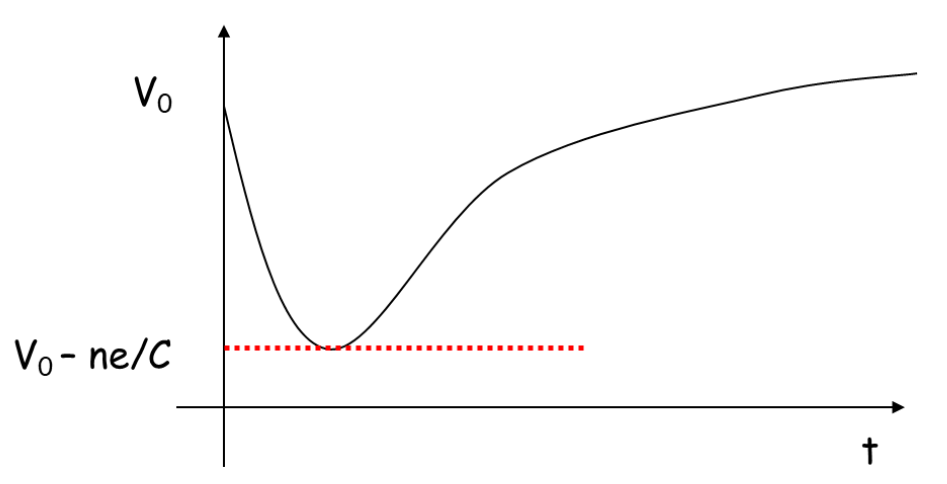
\includegraphics[width=0.6\textwidth]{immagini/impulso_rivelatori_a_gas.png}
   \begin{tikzpicture}
      %assi
      \draw[->] (0,0) -- (7,0) node[right] {$t$};
      \draw[->] (0,0) -- (0,4) node[above] {$V(t)$};
      \draw[red,dashed] (0,0.406) node[left,black] {$V_0 - ne/C$} -- (6.8,0.406);
      \node[left] at (0,3) {$V_0$};
      %grafico
      \draw[thick,teal!80!black] plot[domain=0:2,smooth] (\x, {3*exp(-\x)}) -- plot[domain=0:4.5,smooth] (\x+2, {3*(1 - exp(-\x)) + 0.406*exp(-\x)});
    \end{tikzpicture}
\end{figure}

Ragioniamo ora su che valori deve avere questa costante di tempo.

Se fosse $RC=\infty$, cioè se adoperassimo una resistenza eccessivamente grande, non torneremmo più al valore nominale e quindi la variazione si manterrebbe nel tempo:

\begin{figure}[H]
   \centering
   \begin{tikzpicture}
      %assi
      \draw[->] (0,0) -- (7,0) node[right] {$t$};
      \draw[->] (0,-3.5) -- (0,1) node[above] {$\Delta V(t)$};
      \draw[red,dashed] (0,-3) node[left,black] {$- ne/C$}-- (7,-3);
      %grafico
      \draw[thick,teal!60!black] plot[domain=0:6,smooth] (\x, {-3*(1 - exp(-\x) )}) node[above=0.2cm, black] {$RC=\infty$};
    \end{tikzpicture}
\end{figure}

Chiaramente questa non è una situazione che vogliamo, in quanto vogliamo che a un certo punto si ripristinino le condizioni di partenza in modo da poter essere pronti per una nuova rivelazione.

Facciamo allora un passo indietro: ricordiamo che la raccolta della carica avviene attraverso due fasi successive, perché dapprima avviene la raccolta degli elettroni che sono molto veloci e quindi arrivano subito all'anodo, ma poi abbiamo la migrazione degli ioni che è molto più lenta e quindi comporterà un'ulteriore parte di segnale che corrisponderà a tempi più lunghi. Siccome questo comporterebbe avere un rivelatore molto lento (cioè se volessimo raccogliere tutte le cariche, sia elettroni che ioni, dovremmo aspettare tempi lunghi proprio perché dobbiamo aspettare che gli ioni giungano al catodo), potremmo pensare di accontentarci del segnale prodotto dagli elettroni e quindi potremmo scegliere una costante di tempo tale che il segnale risalga dopo aver raccolto gli elettroni. In altre parole, il valore di $RC$ deve essere compreso tra il tempo minimo necessario a raccogliere il segnale dovuto agli elettroni, $t_{-}$ e il tempo minimo necessario a raccogliere gli ioni, $t_{+}$, cioè $t_{-} < RC < t_{+}$.

Il motivo per cui si trascura quello che fanno gli ioni è che altrimenti si avrebbero dei rivelatori particolarmente lenti. Infatti, nell'ambito della rivelazione parliamo di rivelatori lenti già quando abbiamo tempi dell'ordine dei microsecondi, che sono i tempi necessari per raccogliere gli elettroni, quindi se dovessimo arrivare ai millisecondi la situazione sarebbe ancora peggiore.

\begin{figure}[H]
   \centering
   \begin{tikzpicture}
      %assi
      \draw[->] (0,0) -- (7,0) node[right] {$t$};
      \draw[->] (0,-3.5) -- (0,1) node[above] {$\Delta V(t)$};
      \draw[red,dashed] (0,-3) node[left,black] {$- ne/C$}-- (7,-3);
      \node[left] at (0,-1.5) {$-\frac{1}{2} ne/C$};
      %grafico
      \draw[thick,teal!60!black,join=round] plot[domain=0:0.69314,smooth] (\x, {-3*(1 - exp(-\x) )}) -- plot[domain=0:4,smooth] (\x+0.69314, {3*(1 - 0.5*exp(-\x)) - 3});
      \draw[thick,teal!60!black,dashed] plot[domain=0.69314:6,smooth] (\x, {-3*(1 - exp(-\x) )}) node[above=0.2cm, black] {$RC=\infty$};
    \end{tikzpicture}
\end{figure}

Poiché consideriamo soltanto il segnale che viene generato dalla raccolta degli elettroni, è chiaro che si avranno dei segnali ancora più piccoli in ampiezza, in quanto viene raccolta soltanto metà della carica disponibile; tuttavia i accontentiamo di ciò perché tali segnali risultano più veloci.

\subsection{Il problema della posizione}
Un problema che può sorgere è legato al punto in cui si generano le cariche. Infatti il volume del rivelatore è un volume esteso e in base alla traiettoria che segue la particella queste cariche di ionizzazione potrebbero prodursi in diversi punti della camera.

Schematizziamo l'evento come segue: gli elettrodi si trovano a una distanza $d$ e supponiamo che la ionizzazione avvenga ad una distanza $x$ da un elettrodo, ad esempio quello inferiore:

\begin{figure}[H]
   \centering
   \begin{tikzpicture}
      \draw[thick, black!20!gray] (0,1.5) -- (6,1.5);
      \draw[thick, black!20!gray] (0,-1.5) -- (6,-1.5);
      \draw[thick,-stealth,shorten >= 0.3cm] (-1.5,-0.5) -- (0,-0.5);
      \draw[thick, dashed,red] (0,-0.5) -- (5,-0.5);
      \draw[<->] (6.3,1.5) -- (6.3,-0.5) node[midway, right] {$d-x$};
      \draw[<->] (6.3,-1.5) -- (6.3,-0.5) node[midway, right] {$x$};
      \node at (-1,0.5) {$\displaystyle V=\frac{ne}{C} \frac{x}{d}$};
   \end{tikzpicture}
\end{figure}

In base al valore di $x$, la raccolta del segnale e quindi la tensione che misuriamo ai capi delle armature potrebbe essere leggermente diversa. Il motivo è che le cariche dovranno percorrere uno spazio più o meno grande per arrivare all'anodo, impiegando quindi più o meno tempo. Siccome la costante di tempo, una volta scelta, è fissa, il segnale misurato sarà proporzionale allo spazio percorso, quindi più è grande questo più carica si può raccogliere. Ciò non costituisce un aspetto positivo per la raccolta, perché questo potrebbe portare a dei segnali di ampiezza veramente piccole.

Quello che normalmente si fa per cercare di evitare questo effetto è schermare gli ioni, in quanto il problema nasce dal fatto che scegliamo una costante di tempo opportuna per poter trascurare il segnale dovuto gli ioni.

Se scegliamo una costante di tempo che assicura la raccolta completa degli elettroni e permette di ignorare gli ioni, è possibile andare ad aggiungere una griglia in prossimità del catodo che viene detta \textit{griglia di Frisch} che va a schermare il catodo dall'arrivo degli ioni. Ciò permette di trascurare il segnale dovuto agli ioni e di scegliere una costante di tempo $RC$ anche un po più piccola, permettendo così di ricostruire tutta la carica prodotta indipendentemente dalla posizione in cui avviene l'interazione. 

\begin{approfondimento}[La forma del segnale]
   \footnotesize
   L'approfondimento che segue è sostanzialmente una traduzione di \S 5.VI.B "Pulse mode operation-Derivation of the pulse shape" del Knoll. Lo riporto perché spiega approfonditamente il perché i segnali abbiano quella forma.

   L'analisi della forma dell'impulso prodotto dal flusso di cariche all'interno di una camera a ionizzazione con elettrodi a piastre parallele che sono separati da uno spazio piccolo rispetto alla lunghezza e alla larghezza delle piastre coinvolge una sola variabile: la posizione delle cariche nella dimensione perpendicolare alle piastre. È quindi istruttivo seguire una derivazione semplificata della forma dell'impulso che invoca argomenti basati solo sulla conservazione dell'energia. Questa derivazione fornisce risultati corretti ed evita la complessità matematica che potrebbe oscurare alcuni dei comportamenti fisici importanti nella determinazione delle caratteristiche dell'impulso di uscita atteso in queste condizioni.\\
   Nella derivazione che segue, assumiamo che venga applicato un campo elettrico sufficiente affinché la ricombinazione elettrone-ione sia trascurabile e che le cariche negative rimangano sotto forma di elettroni liberi. Per prima cosa, deriviamo un'espressione per la forma dell'impulso nel caso in cui la costante di tempo del circuito di raccolta sia molto più lunga dei tempi di raccolta di ioni ed elettroni.\\
   La forma dell'impulso dipende dalla configurazione del campo elettrico e dalla posizione in cui si formano le coppie di ioni rispetto alle superfici equipotenziali che caratterizzano la geometria del campo. Per semplificare l'analisi seguente, assumiamo che gli elettrodi della camera siano piastre parallele, per le quali le superfici equipotenziali sono piani uniformemente distanziati paralleli alle superfici degli elettrodi, e l'intensità costante del campo elettrico è data da
   \begin{equation*}
      E=\frac{V}{d}
   \end{equation*}
   dove $V$ è la tensione tra gli elettrodi della camera e $d$ è la loro distanza. Come ulteriore semplificazione, assumiamo che tutte le coppie di ioni si formino a una distanza uguale $x$ dall'elettrodo positivo, dove il potenziale elettrico è uguale a $Ex$. Questa situazione è illustrata nella figura seguente:
   \begin{figure}[H]
      \centering
      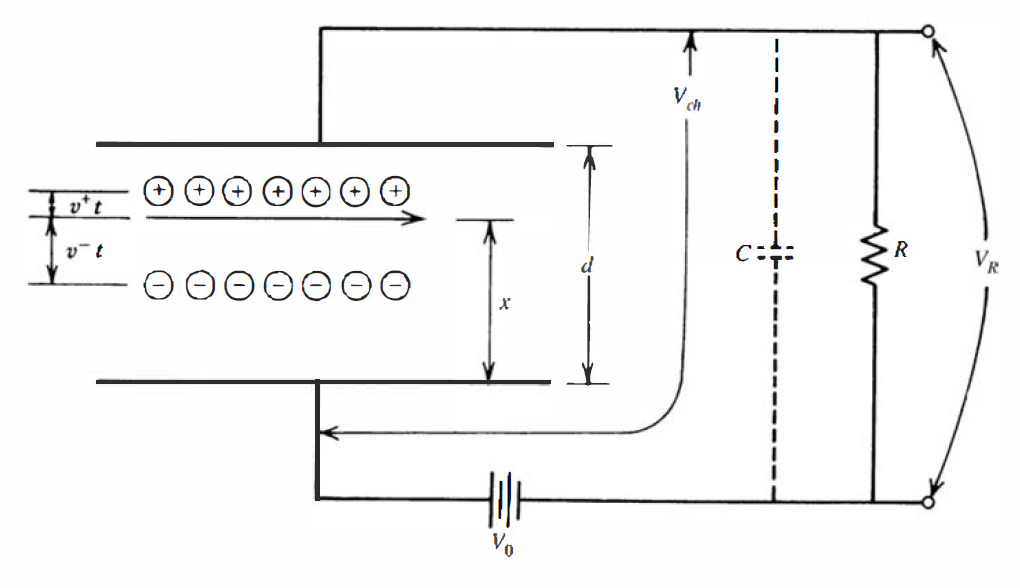
\includegraphics[width=0.6\textwidth]{immagini/circuito_forma_segnale.png}
   \end{figure}
   Poiché si assume che la costante di tempo del circuito esterno sia grande, non può fluire una corrente apprezzabile durante il tempo relativamente breve necessario per raccogliere le cariche all'interno della camera a ionizzazione. Pertanto, l'energia necessaria per spostare le cariche dal loro punto di origine deve provenire dall'energia inizialmente immagazzinata attraverso la capacità $C$, rappresentata dalla camera a ionizzazione. Questa energia è
   \begin{equation*}
      \mathcal{E}=\frac{1}{2}CV_0^2
   \end{equation*}
   dove $V_0$ è la tensione applicata.\\
   Dopo un tempo $t$, gli ioni avranno percorso una distanza $v_{+}t$ verso il catodo, dove $v_{+} $ è la velocità di deriva degli ioni. Allo stesso modo, gli elettroni avranno percorso una distanza $v_{-}t$ verso l'anodo. Entrambi questi movimenti rappresentano lo spostamento di carica verso una regione di potenziale elettrico più basso, e la differenza in energia potenziale viene assorbita nel gas attraverso le molteplici collisioni che i portatori di carica subiscono con le molecole di gas durante il loro movimento. Questa energia è uguale a $Q \Delta\phi$ sia per gli ioni che per gli elettroni, dove $Q$ è la carica totale data da $Q=n_0e$, dove $n_0$ è il numero di coppie di ioni originarie e $e$ è la carica elettronica, e $\Delta\phi$ è la differenza di potenziale elettrico, data dal prodotto del campo elettrico $E$ e della distanza percorsa verso l'elettrodo.\\
   Applichiamo la conservazione dell'energia, che può essere scritta come:
   \begin{gather*}
      \begin{array}{ccccccc}
         \rm Energia &  & \rm Energia &  & \rm Energia & & \rm Energia\\
         \rm immagazzinata & = & \rm assorbita & + & \rm assorbita & + & \rm immagazzinata\\
         \rm iniziale &  & \rm dagli \; ioni &  & \rm dagli \; elettroni &  & \rm finale\\[0.3cm]
         \frac{1}{2}CV_0^2 & = & n_0 e \mathcal{E} v_{+} t & + & n_0 e \mathcal{E} v_{-} t & + & \frac{1}{2}CV_{\rm Ch}^2
      \end{array}
      \\
      \frac{1}{2}C \bigl( V_0 - V_{\rm Ch} \bigr)^2
      =n_0 e \mathcal{E} \bigl( v_{+} + v_{-} \bigr) t
      \\
      \frac{1}{2}C \bigl( V_0 + V_{\rm Ch} \bigr)\bigl( V_0 - V_{\rm Ch} \bigr)
      =n_0 e \qty( \frac{V_{\rm Ch}}{d} ) \bigl( v_{+} + v_{-} \bigr) t
   \end{gather*}
   La tensione del segnale è misurata attraverso $R$ ed è denotata con $V_R$. Essa è quasi sempre piccola rispetto a $V_0$ ed è data da $V_R=V_0-V_{\rm Ch}$. Possiamo quindi fare le approssimazioni
   \begin{equation*}
      V_0 + V_{ch} \approx 2 V_0
      \qqtext{,}
      \frac{V_{\rm Ch}}{d} \approx \frac{V_0}{d}
   \end{equation*}
   Inserendo queste approssimazioni nell'equazione precedente otteniamo:
   \begin{gather*}
      \frac{1}{2}C(2V_0)V_R=n_0 e \qty( \frac{V_0}{d} ) \bigl( v_{+} + v_{-} \bigr) t
      \implies
      V_R=\frac{n_0 e}{d C} \bigl( v_{+} + v_{-} \bigr) t
   \end{gather*}
   Questo risultato descrive la porzione iniziale dell'impulso del segnale e prevede una crescita lineare con il tempo. È valido solo per il periodo in cui sia gli ioni che gli elettroni si stanno ancora muovendo all'interno della camera.\\
   Dopo un tempo $t_{-}=\frac{x}{v_{-}}$, gli elettroni raggiungono l'anodo. La loro deriva ha allora contribuito al massimo possibile alla tensione del segnale, e il secondo termine nell'espressione di $V_R$ diventa una costante pari al suo valore in $t_{-}$. Questo valore costante è $\frac{n_0 e v_{-} t_{-}}{Cd}$ o $\frac{n_0 e x}{Cd}$. Per il successivo periodo di tempo, solo gli ioni si stanno ancora muovendo, e $V_R$ assume la forma:
   \begin{equation*}
      V_R=\frac{n_0 e}{Cd} \bigl( v_{+} t + x\bigr)
   \end{equation*}
   Gli ioni raggiungono il catodo dopo un tempo $ t_+ = \frac{(d - x)}{v_{+}} $. A questo punto, la tensione del segnale non aumenta più avendo raggiunto infine il valore
   \begin{equation*}
      V_R=\frac{n_0 e}{Cd} \bigl[ (d - x) + x \bigr]
      =\frac{n_0 e}{C}
   \end{equation*}
   La forma dell'impulso nei vai intervalli è mostrata nella figura seguente:
   \begin{figure}[H]
      \centering
      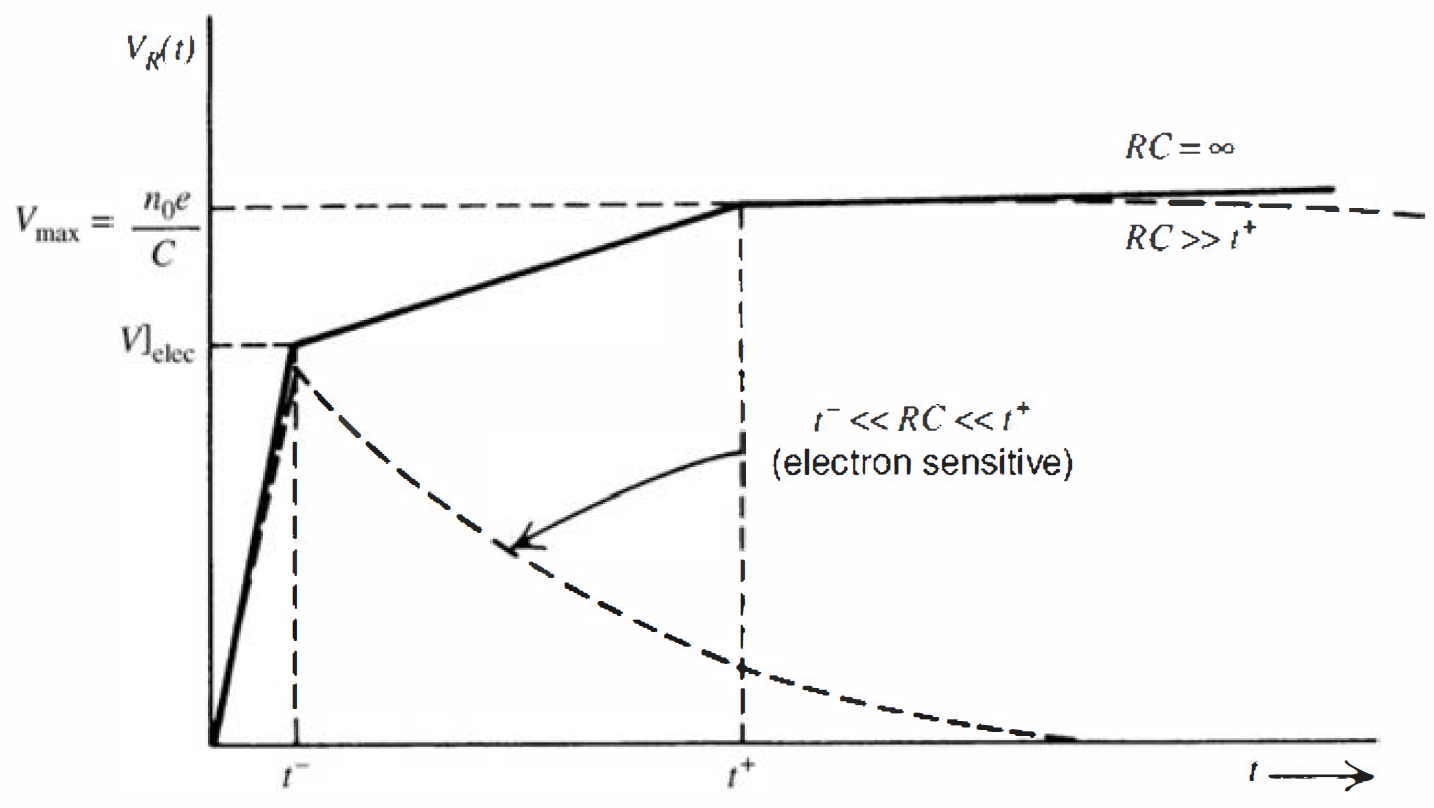
\includegraphics[width=0.7\textwidth]{immagini/forma_segnale_rivelatore_a_gas.png}
   \end{figure}
   Quando la costante di tempo del circuito di raccolta è molto grande, o $RC \gg t_{+}$, l'ampiezza massima dell'impulso del segnale è data da:
   \begin{equation*}
      V_{\text{max}}=\frac{n_0 e}{C}
   \end{equation*}
   e non dipende dalla posizione in cui le coppie di ioni sono state formate all'interno della camera. In queste condizioni, una misura dell'ampiezza dell'impulso $ V_{\text{max}} $ fornisce un'indicazione diretta del numero originario di coppie di ioni $n_0$ che hanno contribuito all'impulso.\\
   Nel funzionamento sensibile agli elettroni, tuttavia, la porzione dell'impulso derivata sopra, che corrisponde alla deriva degli ioni, è quasi completamente persa scegliendo una costante di tempo di raccolta molto più breve rispetto al tempo di raccolta degli ioni. L'impulso che rimane riflette quindi solo la deriva degli elettroni e avrà un'ampiezza data da
   \begin{equation*}
      V_{\text{elec}}=\frac{n_0 e}{C} \frac{x}{d}
   \end{equation*}
   La forma di questo impulso è anch'essa illustrata nella figura sopra. Solo la porzione a crescita rapida dell'impulso è preservata, e l'ampiezza adesso dipende dalla posizione $x$ in cui gli elettroni sono stati originariamente formati all'interno della camera.
\end{approfondimento}

\begin{approfondimento}[La griglia di Frisch]
   \footnotesize
   La dipendenza dell'ampiezza dell'impulso dalla posizione di interazione nelle camere a ionizzazione sensibili agli elettroni può essere eliminata attraverso l'uso di una configurazione illustrata nella figura seguente
   \begin{figure}[H]
      \centering
      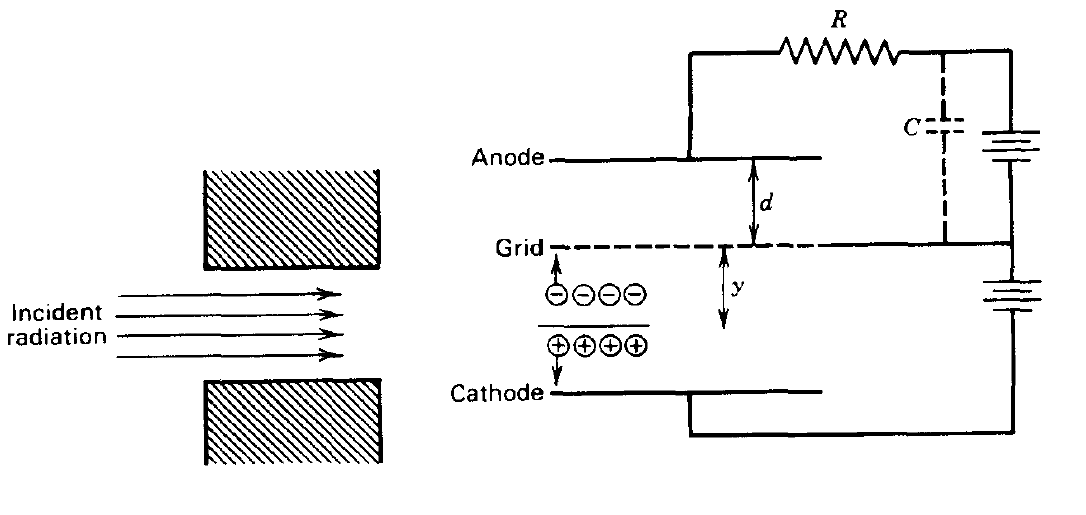
\includegraphics[width=0.7\textwidth]{immagini/griglia_di_frisch_1.png}
   \end{figure}
   In questo caso, il volume della camera a ionizzazione è diviso in due parti da una griglia di Frisch, chiamata così dal suo ideatore.\\
   Attraverso l'uso di una collimazione esterna o della posizione preferenziale della sorgente di radiazione, tutte le interazioni di radiazione sono confinate nel volume tra la griglia e il catodo della camera. Gli ioni positivi semplicemente si muoveranno da questo volume verso il catodo. La griglia è mantenuta a un potenziale intermedio tra i due elettrodi ed è realizzata in modo da essere il più trasparente possibile agli elettroni. Pertanto, gli elettroni sono inizialmente attratti dal volume di interazione verso la griglia. A causa della posizione del resistore di carico nel circuito, né la deriva verso il basso degli ioni né la deriva verso l'alto degli elettroni fino alla griglia producono alcuna tensione di segnale misurata. Tuttavia, una volta che gli elettroni attraversano la griglia dirigendosi verso l'anodo, la tensione griglia-anodo inizia a diminuire e una tensione di segnale inizia a svilupparsi attraverso il resistore. Per una costante di tempo del circuito grande rispetto al tempo di raccolta degli elettroni, il valore di tensione del segnale dipendente dal tempo attraverso il resistore è
   \begin{equation*}
      V_R=\frac{n_0 e}{Cd} v_{-} t
   \end{equation*}
   dove $d$ ora è la distanza tra la griglia e l'anodo. Questo aumento lineare continua fino a quando gli elettroni raggiungono l'anodo:
   \begin{figure}[H]
      \centering
      \begin{tikzpicture}
         \draw[->] (0,0) -- (8.5,0) node[right] {$t$};
         \draw[->] (0,0) -- (0,5) node[above] {$V_R(t)$};
         \draw[dashed] (0,3) node[left] {$\displaystyle \frac{n_0 e}{C}$} -- (7,3);
         \draw[stealth-stealth] (0,4) -- (3.5,4) node[midway,above] {$y/v_{-}$};
         \draw[stealth-stealth] (3.5,4) -- (7,4) node[midway,above] {$d/v_{-}$};
         \draw[dashed] (3.5,4.5) -- (3.5,-0.5);
         \draw[dashed] (7,4.5) -- (7,-0.5);
         %grafico
         \draw[thick, red!70!black] (0,0) -- (3.5,0) node[black,midway, below=0.1cm] {
           $\begin{subarray}{c}
             \text{Gli elettroni si muovono}\\
             \text{verso la griglia}
           \end{subarray}$
         }
         -- (3.5,0) -- (7,3) -- (8.5,3);
         \node[black, below=0.1cm] at (5.25,0) {
           $\begin{subarray}{c}
             \text{Gli elettroni si muovono}\\
             \text{tra la griglia e l'anodo}
           \end{subarray}$
         };
       \end{tikzpicture}
   \end{figure}
   La tensione massima del segnale è quindi
   \begin{equation*}
      V_{\rm max}=\frac{n_0 e}{C}
   \end{equation*}
   che è identico a quella trovata nel caso in cui adoperiamo una costante di tempo $\tau \gg t_+$. Tuttavia, ora il segnale è dovuto solo alla deriva degli elettroni piuttosto che dal movimento sia degli elettroni che degli ioni positivi. L'aumento lento corrispondente alla deriva degli ioni è eliminato, e la costante di tempo del circuito può quindi essere impostata a un valore molto più breve tipico della modalità di funzionamento sensibile agli elettroni descritta nella sezione precedente. Poiché ogni elettrone attraversa la stessa differenza di potenziale e contribuisce ugualmente all'impulso di segnale, l'ampiezza dell'impulso è ora indipendente dalla posizione di formazione delle coppie di ioni originali ed è semplicemente proporzionale al numero totale di coppie di ioni formate lungo la traccia della particella incidente.
\end{approfondimento}

\vfill

\section{La moltiplicazione}

Un'ultimo aspetto da considerare in un rivelatore a gas è la moltiplicazione. La moltiplicazione è una conseguenza dell'aumento del campo elettrico all'interno del gas fino a un valore sufficientemente elevato (si parla di diversi kV/cm). Infatti, per valori bassi del campo, gli elettroni e gli ioni creati dalla radiazione incidente si limitano a migrare verso i rispettivi elettrodi di raccolta; tuttavia, per valori molto elevati del campo elettrico, gli elettroni acquisiscono una velocità estremamente elevata tanto che possono avere un'energia cinetica così grande da poter innescare ulteriori ionizzazioni, che sono delle ionizzazioni secondarie con cui si produrranno ulteriori coppie elettrone-ione.

\subsection{Moltiplicazione a valanga}
L'elettrone liberato da questo processo di ionizzazione secondaria verrà anch'esso accelerato dal campo elettrico. Durante la sua successiva deriva, subisce collisioni con altre molecole di gas neutro e può quindi creare ulteriori ionizzazioni. Il processo di moltiplicazione del gas assume quindi la forma di una cascata, nota come \textit{valanga di Townsend}, in cui ciascun elettrone libero creato in una collisione può potenzialmente creare più elettroni liberi tramite lo stesso processo.

Se $\lambda$ è il cammino libero medio dell'elettrone per una collisione ionizzante secondaria, allora $\alpha=\frac{1}{\lambda}$ è la probabilità di ionizzazione per unità di lunghezza del cammino. Questo è meglio conosciuto come il primo coefficiente di Townsend.

Se ci sono $n$ elettroni, allora in un cammino $\dd{x}$ verrà creato un numero di nuovi elettroni dato da
\begin{equation*}
   \dd{n}=n\alpha\dd{x}
\end{equation*}
Integrando, si ottiene il numero totale di elettroni creati in un cammino $x$ avendo $n_0$ elettroni iniziali (ottenuti dalla ionizzazione primaria):
\begin{equation*}
   n=n_0e^{\alpha x}
\end{equation*}
A partire da tale relazione è possibile definire il fattore di moltiplicazione o guadagno $M$:
\begin{equation*}
   M=\frac{n}{n_0}=e^{\alpha x}
\end{equation*}

\comment{

\subsection{Sviluppo della valanga}

quindi sostanzialmente da una singola prima ionizzazione posso produrre un numero di coppie molto elevato grazie a questi meccanismi di produzione a valanga e questo è capito che è un mandaggio perché avere più carica comporta un segnale più intenso di ampiezza maggiore avevo detto pochi millivolt rispetto attenzioni dell'ordine di centinaia di volte quindi con un meccanismo di moltiplicazione a valanga posso aumentare l'ampiezza del mio segnale prodotto che forma la valanga la possiamo immaginare come una sorta di goccia per il fatto che gli elettroni e gli ioni hanno abbiamo detto velocità molto diverse quindi abbiamo un fronte molto ampio molto popolato da elettroni che si muovono velocemente e poi una coda di ioni che invece si muovono con una velocità molto più bassa quindi se dobbiamo immaginare una valanga la possiamo immaginare con questa tipica forma goccia abbiamo un limite oltre il quale non si va perché appunto potrebbe produrre un danneggiamento del rivelatore perché si incominciano a innescare delle scariche e delle valanghe incontrollate questo è il regime di breakdown che si si supera quando questo fattore di guadagno questo m che abbiamo definito precedentemente supera il valore di 10 alla 8 quindi non possiamo comunque sia produrre un segnale enormemente grande perché poi si si va incontro ad altri fetti indisidirati che sono quelli dovuti al breakdown questa è ad esempio una foto proprio di una valanga quindi vedete la forma tipica della della goccia che abbiamo appena descritto 

\section{Regimi di lavoro dei rivelatori a gas}

concludiamo con questa slide poi vi lascio liberi per provvedere le diverse regioni di funzionamento dei rivelatori a gas quindi adesso mettiamo veramente insieme tutto quello che abbiamo detto il fenomeno della ricombinazione il fenomeno della migrazione e il fenomeno della moltiplicazione in questo grafico vedete riassunte tantissime informazioni abbiamo un grafico che ricorta sull'asse delle ascissse la tensione applicata quindi dovete immaginare un rivelatore a gas con degli elettrodi e appliciamo una differenza di potenziale capite che aumentando la differenza di potenziale aumenta il campo elettrico ovviamente dipende dalla geometria del rivelatore non stiamo a dire che geometria però in generale abbiamo un campo elettrico più intenso sull'asse verticale riportiamo la carica raccolta dagli elettrodi anche se non sono riportati dei numeri su queste scale vi specifico che la scala verticale è una scala logaritmica quindi qui abbiamo dei valori idealmente che variano diversi ordini di grandezza variano parecchio mentre questa sull'asse delle ascissse e una scala lineare allora si individuano diverse reioni cominciamo con la prima regione quando le tensioni applicate quindi i campi elettrici applicati sono abbastanza basse allora in questa regione quello che avviene è che quando passano a particella si producono queste coppie elettrone e ione c'è un campo elettrico ma questo campo elettrico non è molto intenso quindi queste cariche tendono a migrare ma i processi di ricombinazione continuano a prevanere quindi si producono delle coppie ma io non riesco a ricostruire a raccogliere tutte le coppie prodotte perché una parte le perdo a causa dei fenomeni di ricombinazione e questo effetto di ricombinazione diventa di via sempre meno importante man mano che aumenta la tensione perché aumenta la tensione è molto più probabile che la carica riesca a migrare fino all'elettrodo e quindi il segnale raccolto vedete concentrato più soltanto su una curva ad esempio quella rossa il segnale raccolto man mano aumenta fino a raggiungere una pia ne rotto cosa viene in questo pia ne rotto lo sostanzialmente siamo raccogliendo tutte le cariche che sono state prodotte quindi anche aumentando la tensione io già le raccolte tutte le cariche quindi non il segnale non aumenta più di tanto quindi abbiamo una prima regione di pia ne rotto che è la regione in cui funzionano le cosiddette camere a ionizzazione sono dei rivenatori che lavorano in un regime di tensione tale che si raccolvono tutte le cariche prodotte dalla prima ionizzazione supera continuando a aumentare la tensione quello che succede è che si incominciono a innescare i processi di produzione a valanga quindi i campi elettrici diventano così intensi che gli elettroni prodotti dalla ionizzazione primaria possono innescare delle ulteriori iniziazioni e così via quindi mi aspetto che il segnale in cominci ad aumentare quindi il numero di cariche raccolta aumenta e aumenta come secondo la legge abbiamo visto qui con un andamento diciamo esponenziale la legge raccolta aumenta di conseguenza tutta via questa regione se vedete è denominata regione proporzionale per il semplice fatto che anche se abbiamo una produzione a valanga di cariche il numero di cariche prodotte rimane comunque sia proporzionale all'energia depositata quindi se io sono in grado di misurare quante cariche sono prodotte posso comunque sia avere ancora l'informazione sull'energia che è stata depositata nel rivelatore ecco che qui funzionano i cosiddetti contatori proporzionali rivelatori proporzionali quindi abbiamo ancora un'informazione sull'energia depositata cosa succede se andiamo oltre incontriamo una prima regione di proporzionalità limitata quello che avviene in questo caso è che la carica prodotta è così grande quindi abbiamo tanta carica che di goni in particolare vanno a modificare il campo elettrico che ho generato con i miei elettrodi quindi vado in qualche modo a perturbare la proporzionalità che caratterizzava la zona precedente e qui abbiamo quindi una regione che non viene normalmente adoperata per la rivelazione quindi una regione di poco interesse fino a quando non arriviamo a un secondo pienerottolo che il cosiddetto pienerottolo geiger in questo pienerottolo nuovamente abbiamo un segnale che è indipendente dalla tensione di lavoro per quale ragione siamo arrivati una regione in cui si incomincia a nescare delle valange in maniera incontrollata quindi mentre nella regione che avevamo visto in precedenza quindi la regione proporzionale ogni elettrone produceva una nuova valange in gai nescarona e qui si incomincia a nescare lungo l'anodo delle valange che sono in realtà generate da fotoni emessi dalla disecitazione degli atomi che compongono il gas quindi incominciano sostanzialmente a generarsi delle cariche in modo incontrollato e soprattutto il segnale che ho in uscita quindi il numero di cariche che misura alla fine diventa indipendente da quante cariche sono state prodotte all'inizio della prima ionizzazione quindi dall'energia che sarà depositata insomma il segnale in uscita non mi da più alcuna informazione sull'energia depositata nel rivelatore quindi sembra ovviamente una regione diciamo meno interessante perché abbiamo dal segnale meno informazioni non possiamo sapere l'energia di depositata ma possiamo sapere se è passato meno una particella ecco perché questa regione in questa regione funzionano i contatori quindi delle rivelatori che permettono solamente di contare quante particelle sono passate senza fornire indicazioni sull'energia e tra questi contatori abbiamo appunto il contatore geiger miller subito dopo questa regione che è un piano rotto che in realtà comunque siamo a leggerissima tendenza abbiamo una regione di scarica continua quindi questo ovviamente la regione da evitare perché potrebbe produrre dei danneggiamenti del rivelatore quindi in un solo grafico abbiamo individuato le diverse reioni di operatività di un rivelatore a gas in particolare abbiamo detto la prima regione non viene la doverata perché ci sono effetti di ricominazione aumentando la tensione abbiamo le camera ionizzazione poi abbiamo la regione proporzionale dove incominciano a prodursi a valanga processi di ionizzazione secondaria abbiamo una regione di limitata proporzionalità che non ci interessa scopi della rivelazione infine abbiamo il piano rotto log geiger quindi da questo grafico individuiamo tre tipologie di rivelatore a gas camera ionizzazione camera proporzionali e rivelatori geiger 

%va bene ragazzi ci fermiamo qui per oggi noi ci vediamo giovedì giovedì pomeriggio saluto anche ragazzi da casa stacco la connessione a rivederci ah scusate ma ci sono domande non ho scusata vogliamo controllare le partigielle di riferimento di rivelatore e come la mia vizionazione avventano lo del abbiamo un zone dove abbiamo questo condizionato questo è un latte che ci fanno da unlicato le sue placche non tenete in un zone in cui la particella non interagisce Sony che si trattano, si trattano, si trattano come la particella diretta del sceglielo del gasse. Allora sì, chiaramente poi la geometria la vedremo bene nel dettaglio e quando abbiamo un rivelatore ci sono delle finestre di ingresso. Ok quindi soprattutto perché alcune tipologie di particelle come ad esempio in beta o le alpha maggior ragione perdono energia banalmente anche nell'attraversare spessori piccoli, ecco perché in alcuni rivelatori si creano non solo delle aperture perché il contenitore deve essere ovviamente attenduta, ma ci sono delle pareti che sono realizzati con particolari materiali ad esempio pareti di mica, cioè un materiale in cui la perdita di energia è molto bassa. Quindi ci sono delle reioni preferenziali di rivelazione rispetto ad altre. Poi ci sono altri tipi di particelle che non vengono giuensate dalla presenza di elettro di che possono essere esempio pieno paralleli oppure poi vedremo la geometria cilindrio quindi immagina un cilindro addirittura che rappresentano un elettro. In questi casi ad esempio le nuoni mettiamo non vengono totalmente, si riescono a passare quindi non ha alcuna importanza. Però per altre particelle è importante avere una finestra di ingresso quindi una zona del rivelatore che facilita l'ingresso delle particelle senza far perdere energia. E chiaro che ad esempio una particella alpa non riuscirebbe mai ad attraversare un elettro ed entrare nella camera. 

\textbf{lez 11}

proseguiamo con i rivelatori a gas che avevamo iniziato a vedere la volta scorsa e avevamo iniziato con questi rivelatori perché sono i più semplici in assoluto e la volta scorsa se vi ricordate abbiamo discusso i diversi processi che possono avvenire all'interno di un gas abbiamo detto che i rivelatori a gas sono dei contenitori dei recipienti riempiti di un opportuno miscela di gas spesso si utilizzano dei gas nobili e il principio di base è la ionizzazione quindi una particella una radiazione che entra all'interno del rivelatore poi ionizzare il gas quindi produrre coppie elettrone ion e positivo e sono queste quelle che noi dobbiamo andare a raccogliere per creare un segnale elettrico che ci dice che è passato una particella attraverso il rivelatore e addirittura in determinate condizioni siamo anche in grado di misurare l'energia che è stata depositata all'interno del rivelatore perché questo numero di coppia che l'abbiamo visto è legato a quante energie è stata depositata perché in media ci vogliono in circa una trentina di eV per produrre una coppia elettrone e ione e conoscendo esattamente questo questo valore quindi l'energia media per creare una coppia possiamo risalire a quante energie è stata depositata andando a misurare il numero di coppie prodotte in realtà il tutto è un attimino più complesso perché all'interno del rivelatore dobbiamo andare a creare un campo elettrico perché queste coppie ovviamente se le lasciamo lì dove si sono formate si muovono ovviamente per agitazione termica però prima o poi ci riconvinano e quindi dobbiamo in qualche modo farle migrare verso del zone del rivelatore dove è possibile andare a raccogliere il segnale elettrico e per questo motivo creiamo un campo elettrico con degli opportuni elettrodi e se vi ricordate la volta scorsa ci siamo lasciati discutendo questo grafico che riassume molto bene il principio di funzionamento dei principali rivelatori al gas abbiamo detto tutto dipende dal campo elettrico che stiamo creando all'interno del rivelatore infatti sull'asse delle schisse se vi ricordate è riportata la tensione applicata in qualche modo il campo elettrico dipende dalla tensione ovviamente dipenderà in base alla forma degli elettrodi quindi un discorso di avere delle ad esempio degli elettrodi piani e paralleli oppure un altro discorso di avere una geometria cilindrica comunque in generale ci interessa semplicemente dire che man mano che la tensione ci aspettiamo valori di campo elettrico più intensi mentre sulle ordinate riportiamo la carica raccolta in scala 

logaritmica e abbiamo evidenziato diverse reioni se vi ricordate la rima regione è una regione che non viene utilizzata per la rivelazione perché abbiamo dei campi elettrici così poco intensi che le cariche incominciano a migrare per effetto del campo elettrico però il campo elettrico non è sufficiente e quindi una parte di queste cariche vengono perse perché si riconvinano chiaramente questo effetto di riconvinazione diventa sempre meno importante quanto più è elevato il campo elettrico quanto più è elevata la tensione ecco perché man mano in questa prima zona di questo grafico e il numero di cariche raccolte ovviamente aumenta con la tensione arriviamo a un un piani rotulo siamo nella regione di ionizzazione quelle dove un quello dove funzionano le camera e ionizzazione e vi ricordo che in questa regione tutte le cariche prodotte per ionizzazione prima maria vengono raccolta gli elettrodi ecco perché anche aumentando la tensione non raccogliamo più cariche di quelle che sono state prodotte e quindi abbiamo una dipendenza molto plebide del segnale raccolto della tensione applicata segue una zona di proporzionalità dove se vi ricordate il campo elettrico è così così da accelerare gli elettroni e far sì che questi elettroni abbiano un energia tale da produrre ionizzazioni successive secondaria quindi si formano una sorta di valange a seguito di questi elettroni energetici e in particolare continuiamo a mantenere una proporzionalità col numero di elettroni primari prodotti dalla ionizzazione primaria infatti se vi ricordate definire un coefficiente di guadagno un fattore di moltiplicazione e da questa relazione vedete che il numero di cariche prodotte dopo un certo percorso x è dato dal numero di elettroni prodotti durante la prima ionizzazione per e in alzato dal fa x quindi abbiamo vedete una proporzionalità tra n e del n col 0 e questo ci permette questa regione di dire che se raccogliamo il segnale possiamo andare a conoscere l'energia depositata quindi una regione in cui i rivelatori sono in grado di fornire ancora delle informazioni sull'energia depositata dalla particella e questa è la regione proporzionale dove dove lavorano i contatori proporzionali dopo di che abbiamo una regione in cui questa proporzionalità in comincia a mancare perché il campo elettrico presente nel rivelatore viene modificato a seguito della enorme densità di carica che si sta producendo all'interno del rivelatore e quindi questa regione in realtà non viene utilizzata a scopi di rivelazione e poi ci 

ritroviamo un ultimo piene rottolo che è detto piene rottolo geier muller dove appunto operano questo tipo di rivelatori e è una regione in cui si innescano delle balange all'interno del gas che però non sono originate direttamente dagli elettroni prodotti dalla ionizzazione primaria infatti a seguito di emissione di fotoni all'interno del gas perché le molecore si disecitano questi fotoni possono innescare delle nuove scariche delle nuove valange e quindi perdiamo sostanzialmente il controllo della produzione di queste valange il segnale in uscita diventa indipendente da quante cariche primarie si erano prodotte e quindi vedete questo piene rottolo che tuttavia viene sfruttato per la rivelazione che informazione perdiamo quella sull'energia perché a questo punto indipendentemente dall'energia depositata si produce sempre lo stesso segnale l'unica cosa che ci interessa in questa regione è il fatto che si produca il segnale quindi questi rivelatori indicano il passaggio di una particella permentano di contare quante particelle passano ma non ci dicono nient'altro sulla natura o sull'energia di questa particella se guardiamo questo grafico presenta diverse curve una è stata riportata per una particella alfa all'interno di un rivelatore al gas una particella beta è un $\gamma$ quindi vi fa vedere grosso modo qual è il segnale rilasciato parità di tensione di lavoro quindi il segnale è rilasciato da queste cariche e da questa radiazione vedete per il $\gamma$ la carica prodotta è più bassa in generale alfa e beta si differenziano dipendono ovviamente dallo stop in power di queste particella all'interno del gas ma la cosa che ci interessa di più al di là dell dell'ordine con cui si presentano queste curve andrà a vedere vedere le curve sono ben distanziate finché lavoro nella regione delle camera ionizzazione o dei contatori proporzionali ma poi si unificano e in corrispondenza del contatore gaider vedete che non c'è più alcuna distinzione quindi indipendentemente dal tipo di particella indipendentemente dell'energia che è stata depositata all'interno del rivelatore il segnale in uscita è sempre lo stesso quindi questi sono dei contatori veramente basilari non danno altre informazioni se non il fatto che è passato una particella come vi dicevo prima il campo elettrico che si genera all'interno del rivelatore dipende dalla geometria del rivelatore una geometria molto semplice è quella costituita da due lettro di affacce piano e parallele quindi sostanzialmente un rivelatore di questo tipo lo possiamo schematizzare come se fosse un condensatore affacce piano e parallele quindi all'interno di questo volume tra le piastre abbiamo il nostro gas le piastre sono distanziate da 

una distanza di e applichiamo una differenza di potenziale tra una piasta e l'altra sapete benissimo dalla fisica 2 che il campo elettrico che si genera in questa regione compresa tra i due elettro di e un campo elettrico uniforme di valore di sud di questo tipo di geometria viene normalmente doperata nelle camera ionizzazione quindi in questa regione dove la tensione non è molto elevata ok quindi non ci aspettiamo campi elettrici particolarmente elevati immaginato ad esempio di applicare qualche centinaia di volt su un condensatore affacce piano e parallele con le armature distanti qualche centimetro vuol dire che se andiamo a vedere questa formula il campo elettrico che si produce è dell'ordine di 100 volt per centimetro in grosso modo come ordine di grandezza quindi non sono campi elettrici particolarmente intensi infatti i segnali che si producono in questo questo di rivelatori sono segnali piccolini l'avevamo fatto anche un esempio se vi ricordate la lezione scorsa supponendo una determinate estensione di queste di queste rastre una determinata superficie una determinata distanza abbiamo valutato la capacità e abbiamo fatto un conto che ci ha portato a dire che il segnale che ci aspettiamo è dell'ordine dei millivolt rispetto alle centinaia di volte che ben non applicate alle armature quindi sono segnale abbastanza deboli cosa possiamo fare se vogliamo avere dei campi elettrici più intensi capite se manteniamo la geometria di prima per aumentare il campo elettrico dovremmo o aumentare la tensione o diminuire la distanza tuttavia la geometria che vi sto facendo vedere qui è il limitativo allo stesso perché si potrebbe arrivare a superare quello che è la rigidità di elettrica del mezzo e quindi si potrebbe arrivare alla condizione di scarica che ovviamente una condizione da evitare come facciamo a produrre campi elettrici intensi nella regione di rivelazione basta da muovire geometria e quindi si adopera la geometria cilindrica nella geometria cilindrica abbiamo sostanzialmente sempre due elettrodi allora un elettrodo e il cilindro esterno di raggio in questo caso b l'altro

elettrodo è un filo che corre lungo l'asse del cilindro ovviamente il filo alle sue dimensioni non è un filo di dimensioni infinite infinitamente piccole ma avrà anche esso un raggio che è indicato in questo caso con la riterra a tra i due elettrodi quindi tra il cilindro esterno e il filo interno viene creato una differenza di potenziale quindi vedete in questo schema il cilindro esterno è collegato a massa mentre il filo interno è posto a un potenziale più di con zero quindi il filo rappresenta l'anodo il cilindro esterno rappresenta il catodo il principio di funzionamento è esattamente lo stesso quindi passa una particella produce ionizzazione primaria questa volta abbiamo dei campi elettrici molto intensi e quindi si generano delle valange addirittura potremmo arrivare a lavorare nella modalità geiger dove queste valange sono incontrollate sostanzialmente e il segnale è uscita e nipendente dalla particella dell'energia depositata perché il campelettrico è molto intenso perché se vi ricordate la formula che esprime il campo elettrico ha una certa distanza radiale dal filo questo campelettrico è dato ovviamente della differenza di potenziale tra i due elettrodi ma dipende da r quindi dalla distanza dal filo quindi in prossimità del filo ovviamente il campo elettrico diventa molto intenso addirittura per r uguale a zero diventerebbe infinito e dipende dalle caratteristiche geometriche di questo cilindro in particolare dai raggi interno del filo interno e del cilindro esterno attraverso questo logaritmo di b su a dove vi ricordo che b è il raggio del cilindro esterno e a è il raggio del filo che attraversa il rivelatore quindi in prossimità dell'anodo si possono raggiungere valori di campelettrico particolarmente intensi vediamo questi esempi numeri con supponiamo ad esempio che il lano ado abbia un raggio di 0,01 centimetri quindi un decimo di millimetro e che il raggio invece del cilindro esterno sia di un centimetro sono dimensioni abbastanza realistiche. 

Applichiamo una differenza di potenziale questa volta di un miliario di volt e se vi fate il conto in corrispondenza dell'anodo in prossimità dell'anodo il campelettrico arriva a raggiungere anche valori di 20 kV per centimetro quindi molto più elevati rispetto a quelli che possiamo ottenere con la geometria a faccepiene parallele. Il segnale che si genera è di conseguenza un segnale molto elevato possiamo dire anche dell'ordine del volt sempre da confrontare con i mille volt di differenza di potenziale che noi adoperiamo tra gli elettrovi e questa è la classica geometria di un contatore geiger quindi alla fine uscirà da questo rivelatore un segnale abbastanza ampio che ci dice se è passata o meno una particella quindi quando si verifica un segnale in uscita vorrò dire che è passata una particella quindi all'interno abbiamo queste valange che fanno sì che il segnale diventi indipendente dell'energia depositata ed è un po quello che è schematizzato in questa figura vedete qui abbiamo il nostro elettrone prodotto dalla ionizzazione primaria elettrone asselute del campelettrico viene accelerato e riesce a produrre a sua volta ionizzazioni secondarie quindi produce questa valanga ma se vedete lungo l'anodo ci sono tantissime altre valange che in realtà non derivano da un elettrone di ionizzazioni primaria ma derivano da questi fotoni che vengono a messi asseluto della disecidazione delle molecole quindi sono correlati in qualche modo alla prima valanga ma perdiamo completamente la proporzionalità che caratterizzava la prima regione di lavoro dei rivelatori il contatore geiger quindi lavora in questa regione in questo piano e rotto la prende il nome proprio di piano e rotto lo geiger che in realtà ha una leggera pendenza dell'ordine di 2 3 per cento per volta cioè il segnale però ogni volta può cambiare del 2 3 per cento che non è tantissimo ovviamente però è un piccolo aumento quello che si fa quando si lavora con un contatore geiger e cercare di capire la tensione di lavoro ottimale quindi a quale valore di differenza di potenziale bisogna porre il elettro di il contatore geiger per lavorare all'incirca al centro di questo piano e rotto perché capite che bisogna evitare di lavorare in prossimità dell'estremità del piano e rotto perché in questo caso entriamo in due reioni di lavoro che noi vogliamo evitare da un lato abbiamo la 

regione di breakdown dove si innescano delle scariche tra gli elettro di ed è una regione in cui il rivelatore può anche danneggarsi dall'altro lato sulla sinistra invece ci troviamo la regione quella di limitato proporzionalità che anche può essere una regione che non ci interessa ai fini della rivelazione e quindi bisogna con il contatore geiger man mano aumentare la tensione e verificare quando si raggiunge il piano e rotto lo e cercare di doperare una tensione di lavoro in prossimità del centro del piano e rotto lo cosa può rivelare un contatore geiger questo vale un po in generale anche per altri rivelatori a gas chiaramente particelle cariche questo certamente perché le particelle cariche ionizzano la materia e l'unica attenzione che dobbiamo avere riguarda l'ingresso all'interno del rivelatore perché chiaro che il rivelatore è un recipiente che è chiuso ermeticamente perché abbiamo un gas quindi dobbiamo tenere il chiuso ermeticamente quindi a delle pareti e queste pareti devono essere necessariamente attraversate delle particelle se queste devono essere rivelate ora finché abbiamo che fare ad esempio con elettroni, gli elettroni comunque si hanno un potere penetrante diciamo abbastanza discreto e quindi se si realizzano delle finestre sottili, delle finestre di ingresso sottili quindi una delle pareti del contatore geiger viene realizzata con materiale magari con un basso stopping power particolarmente sottili con densità bassa allora l'elettrone può penetrare all'interno del rivelatore e magari perde una piccola parte della sua energia per comunque si riesce a entrare all'interno del rivelatore e quindi possiamo dire ad esempio che nel caso il contatore geiger l'efficienza di rivelazione per gli elettroni e dell'ordine del 100\% se vi ricordate la omodefinita l'efficienza in trince che rappresenta il rapporto tra il numero di particelle rivelate e il numero di particelle incidenti quindi la particelle incide viene rivelato oppure no riesce a entrare nel rivelatore per un urno segnale consistente oppure no e questo rapporto quindi ci dà le efficenze questo caso tutti gli elettroni che incidono sul contatore geiger possiamo dire che vennero rivelati un'efficienza di trince da 100\% per per 100. Il raggi $\gamma$ qui la situazione è un po' diversa se vi ricordate il raggi $\gamma$ interagiscono attraverso meccanismi diversi sicuramente non ionizzano la materia e quello che possono fare è produrre effetto fotoelettrico effetto conto produzione di coppie quindi eventualmente sono i prodotti carichi di queste interazioni che possono ionizzare il gas quindi se ad esempio avviene effetto fotoelettrico sarà l'elettrone messo per effetto fotoelettrico che può ionizzare il gas quindi affinché il $\gamma$ venga rivelato è necessario che interagisca allora è molto probabile che possa interagire con le pareti perché le pareti hanno una densità o uno z elevato è più difficile che il $\gamma$ interagisca con il gas stesso sia per una questione di densità sia per una questione di z di numero atomico del gas quindi l'efficienza nel caso del raggi $\gamma$ è un po' più basso perché il $\gamma$ deve interagire con le pareti del 

materiale e i prodotti di questa interazione devono poi da produrre un segnale del contatore geiger altre particelle che vi troverete a misurare con contatori geiger sono i consnici i moni consnici ma i moni sappiamo che hanno un elevato potere teleprante quindi riescano ad attraversare tranquillamente le pareti del recipiente senza essere schermati o assorbiti che cosa ci rimane da questo schema le particelle alfa o comunque in generale particelle cariche pesanti è qui la situazione è più difficile perché se vi ricordate le particelle cariche pesanti percorrono spessori di materiale solido veramente piccoli e poi vengono fermate quindi bastano una cinquantina di microle di silicio per arrestare una particella alfa da un mezzo quindi capite che una qualsiasi parete alla fine arresterebbe le particelle alfa comunque farebbero perdere gran parte dell'energia di queste particelle quindi è veramente difficile misurare particelle alfa con il contatore geiger quindi il laboratorio vi dicevo ad operare dei geiger per la misura di elettroni ma vi far fare anche una esercitazione che non fa parte delle esperienze di esame quindi non farete una tesina non verrà estratto come tesina ma è un'esercitazione sulla statistica di posto attraverso la rivelazione della radiazione posmica con i contatori geiger e la farete in questo primo gruppo di esperienza esistono in realtà altre geometrie che permettono di realizzare dei campi elettrici intensi quindi non solamente la geometria cilindrica che abbiamo descritto adesso ma anche altre geometrie come adesso più quelle che vedete qui è riportato anche qua sotto il la descrizione il nome comunque di queste geometrie ad esempio questo è il parallel plate strip col groove insomma sono diverse ma non entraremmo nel dettaglio tutte queste linee che vedete rappresentano le linee del campo elettrico e comunque si riescono vedete a generare delle zone secondo un campi elettrici molto elevati lo vedete dalla densità di linee del campo elettrico anche con altre geometria A questo punto parliamo brevemente di alcuni rivelatori un po' più moderni. Infatti vi ho detto quei rivelatori sono rivelatori storici, possiamo dire, i primi rivelatori che sono stati sviluppati. In particolare i contatori guider vengono adoperati più per scopi didattici dimostrativi, perché sono dei rivelatori molto semplici, ci sono delle versioni portatili, i contatori proporzionali o le camera ionizzazioni sono più che altro applicate, utilizzati in alcune applicazioni, soprattutto nel campo medico. Nel campo della ricerca si adoperano dei rivelatori diversi e ne vedremo alcuni questo pomeriggio. Qua abbiamo riportato delle sì che le ma comunque ora li vediamo a poco a poco. Una prima tipologia di rivelatori a gas un po' più moderno è il cosiddetto Multiwire Proposional Chumbers. 

Queste sono state sviluppate intorno agli anni 70 e, sostanzialmente, si comportano come un insieme di contatori proporzionali. Quindi vedete da questa animazione cosa viene all'interno di una camera di questo tipo. Innanzitutto abbiamo due piani, vedete qui uno sopra e uno sotto, e sono entrambe dei catodi, quindi sono delle superfici piane. Poi abbiamo il centro, all'interno della camera, diversi fili che rappresentano gli anodi. Chiaramente stiamo vedendo una sezione di questa camera, quindi dovete immaginare come se il filo entrasse all'interno dello schermo che state vedendo. Ok, quindi sono state vedendo una sezione. Quello che avviene, ovviamente, è quello che avviene all'interno di un qualsiasi rivelatore a gas, quindi vedete una particella che entra, produce delle coppie, elettrone, lione e positivo per rivelizzazione, e gli elettroni viaggiano verso l'anodo, mentre gli ioni positivi verso il catodo. La vediamo nella regione di proporzionalità, quindi vedete arrivati a un certo punto in prossimità dell'anodo, dove il campanettico è molto intenso, gli elettroni sono in grado di produrre ionizzazioni secondarie. E quindi aumentano davvero il numero di questi elettroni. Dove vanno questi elettroni? Idealmente vanno verso il filo più vicino. Quindi se la particella incide vicino questo filo, il segnale verrà raccolto da questo filo. In questo caso non si va a misurare l'ampiezza del segnale, quindi non si è interessata quante cariche sono state prodotte, ma semplicemente ci limitiamo a vedere quale filo ha raccolto il segnale, perché questi rivelatori sono rivelatori di posizione, quindi permettono di ricostruire la posizione di incidenza della particella. In questo caso lungo una sola direzione, ovviamente, perché se la posizione è data dal filo, capite che la coordinata che sto andando a ricostruire è quella parallela ai piani dei catoli, che è quella che sto indicando con il mouse. E la prima volta che forse incontriamo un rivelatore di posizione, quindi un rivelatore che fornisce tra le informazioni possibili la posizione della particella. Capite che in questo caso viene ricostruito una sola coordinata, ma banalmente basta utilizzare due di queste camere, una sopra naltra in maniera tale che i fili siano ortogonanica di loro, per poter andare a ricostruire anche un'altra direzione nel piano XY. L'informazione che vi dicevo che viene stratte semplicemente è un'informazione del tipo SIDNO, eventualmente un miglioramento si potrebbe avere se la carica viene raccolta magari da due fili contigui, allora in quel caso capite che si può realizzare una sorta di baricentro. Vedete qui una geometria tipica, questi sono i due catodi che abbiamo visto prima, questi sono gli anodi e vedete queste linee rappresentano il campo elettrico, quindi nella maggior parte della camera il campo elettrico è uniforme, chiaramente in prossimità del filo il campo elettrico diventa molto più intenso e tipicamente si potrebbe avere ad esempio fili da 20 micro, non spaziati da un millimetro come distanza, la distanza tra un filo e l'altro prende il nome di pitch, ma questa è una caratteristica di tutti i rivelatori segmentati, quindi la distanza tra un elettro del successivo prende il nome di pitch. Ed è importante conoscere il pitch di un rivelatore in posizione, perché questo stabilisce politica la risoluzione spaziale. Fino a questo noi abbiamo parlato di risoluzione energetica di un rivelatore, cioè la capacità di distinguere due valori in energia vicini tra di loro. Poi abbiamo parlato di risoluzione temporale, quindi la capacità la parte di un rivelatore, di produrre un segnale che gli da una informazione di timing per ad esempio effettuare misure di tempo di volo. Adesso abbiamo visto dei rivelatori in grado di costruire la posizione, quindi siamo interessati a un'altra caratteristica, la risoluzione spaziale. Quindi la capacità di andare a distinguere due posizioni molto vicine tra di loro, quindi la precisione con cui viene ricostruita questa coordinata spaziale. E allora banalmente voi capite che questa deve dipendere da quanta distanza c'è, tra in questo caso un filo e il successivo. 

E' chiaro che se i due fili fossero distanziati da 10 cm, io non posso dire niente su quello che avviene in questi 10 cm, al massimo appunto assegno la posizione a un filo o all'altro. Quindi più sono fitte queste sequenze di fili, migliore sarà la risoluzione spaziale. Però la risoluzione spaziale non è banalmente la distanza tra un filo e l'altro, quindi in questo caso un milidimetro. La risoluzione spaziale si può dimostrare è data da questa distanza diviso alla radice di 12. Quindi ad esempio per di pari 1 mm si possono ottenere risoluzioni spaziali dell'ordine di 0,3 mm. Questa è una foto prezzo da un archivio storico del CERN, dove si vedono tre fisici al lavoro di una camera fili, forse non si percepiscono i fili perché sono molto piccoli, però tutti queste camera sono in Italy che vanno a permettere di distendere questi fili. Tra questi fisici in particolare possiamo vedere il Charpack, che è un fisico che ha vinto un premio Nobel proprio per l'invenzione di questa tecnica di rivelazione. Come mai viene fuori questa risoluzione spaziale con questo fattore radice di 12? Si può spiegare diversi modi. Un modo che possiamo provare a mostrare è questo. Immaginate di avere una distribuzione uniforme, cioè queste particelle, quando arrivano sul rivelatore. Io immagino che non ci sono altre motivazioni di base, immagino che arrivino con la stessa probabilità in qualsiasi punto della superficie del rivelatore. Quindi se devo andare a immaginare tra un filo e l'altro, qual è la funzione che descrive la distribuzione di probabilità di queste particelle, o comunque della posizione di queste particelle, mi aspetto che sia una funzione di probabilità fiatta, uniforme. Una volta definita la funzione di distribuzione di probabilità che chiamiamo pdf, sapete che, dato una distribuzione di valori, possiamo valutare valore medio e varianza. Il valore medio lo calcolate banalmente come l'integrale di x, che è la mia variabile, in questo caso la mia posizione lungo quell'as, per la funzione pdf, index. Evidentemente si divide per l'integrale di x, index, se questa funzione pdf non è normalizzata a uno. Però se è normalizzata a uno, addirittura questo rapporto non è necessario. Quindi questa è la definizione di media di una distribuzione, o comunque di una funzione di dx. La varianza, se vi ricordate, è l'integrale di x, meno x media al quadrato, per dx, index. Al solito possiamo dividere per l'integrale della funzione dx, se questa non è normalizzata a uno. Quindi semplicemente qua stiamo usciendo un discorso generico, data una distribuzione indicata da questa funzione di x, calcolo valore medio e varianza. Quindi vi sto ricordando soltanto queste formula. A questo punto facciamo il caso concreto. Questo è il nostro rivelatore segmentato. Quindi tutte le particelle che cadono, ad esempio nell'intervallo 2, verranno associate a questo filo. Sto facendo un esempio della camera a fili, ma vale, capite, per qualsiasi rivelatore segmentato, quindi dove abbiamo degli elettroni segmentati. Quindi questo corrisponde ad esempio al filo 2. Quindi tutte le particelle che eritavano in questa regione vengono associate come posizioni al filo 2. Abbiamo detto che queste particelle, io mi aspetto, si distribuscono in maniera uniforme. Quindi la loro distribuzione di probabilità deve essere piatta. Allora la posso esprimere questa funzione. Vedete nel seguente modo tra l'estremo A e l'estremo B, che sono gli estremi, entro cui io suppongo di associare il filo 2 alla particella. Questa funzione può assumere l'espressione 1 sub b meno a. Vedete anche normalizzata 1, perché se fate l'integrale tra A e B di questa funzione, questo fa esattamente 1. Mentre è 0 in tutti i altri canali, quindi per adesso vi sto concentrando solamente su questo aspetto. Calcoliamo il valor medio. Non ho riportato i conti, ma se fate un conto a mente, perché un integrale è veramente semplice, perché dovete prendere questa funzione e moltiplicarla per x, quindi avrete l'integrale di x sub b meno a in de x, integrale tra A e B. Quanto verrà, ovviamente, varrà il valore medio a più b diviso 2. Vi possiamo fare il conto malalmente. Ad esempio qui, se questa corrisponde alla posizione 2, e questa sarà 1 e mezzo e queste 2 e mezzo, capite che il valore medio sarà 2. Questo viene fuori matematicamente. Per la varianza magari c'è qualche passaggio in più, e qui vi faccio vedere la varianza, comunque non entriamo a le tagli del conto, che è un semplicissimo integrale, poi scasomevo i valori vedete nel slide. Quello che si succede, per questa varianza alla fine, risulta essere pari a b meno a al quadrato diviso 12. Insomma, la devienzione standard di questa distribuzione è proprio b meno a diviso radice di 12. Questo spiegha l'origine di quel fattore radice di 12 che abbiamo visto nella risoluzione. Un altro modo è anche fare voi stessi, verificare voi stessi con un valore, con un foglio Excel, io quello ho fatto corrutto, e generare un certo numero di numeri casuali, in modo uniforme, quindi una distribuzione uniforme tra due estremi. Ad esempio io qui ho scelto come estremi il valore 1 e 5 e 2 e 5, e ho generato 100.000 numeri in modo uniforme. Vedete la distribuzione è abbastanza piatta di questi valori, è chiaro non è perfettamente piatta per questioni di statistica, per situazioni statistiche, però vedete che è qui probabile che una particella abbia colpisca rivalatore in corrispondenza della coordinata 1 e 6, lo colpisce nella posizione 2 e 4, quindi stessa probabilità. Se andate a calcolare il valore medio di questa distribuzione, vedete in questa box con la statistica, il valore medio viene 2, come ci aspettavamo, e il centro di questa distribuzione. L'RMS, quindi ad evitazione standard, 0,29, se vi fate il conto corrisponde proprio a 2,5, meno 1,5 in isolarice di 12, quindi questa è una verifica a posteriori di quello che abbiamo dimostrato matematicamente, però lo possiamo fare anche in Excel e vi viene fuori esattamente questo risultato. Che è una conseguenza alla fine del teorema del limite centrale, che ci dice che la somma o la media di un gran numero di variabili casuali, aleatorie, indipendenti tra di loro, serve una distribuzione da ossiana, con ad evitazione standard data da questa espressione. Alla fine quando noi 

andiamo ad assegnare il centro di questo intervallo a qualsiasi particella che incide entro questi limiti, vuol dire semplicemente supporre che vado a considerare il valore medio. E quindi se il valore medio ha una distribuzione normale con questa deviazione standard, posso supporre come precisione nella ricostruzione della posizione il valore di questa deviazione standard. Quindi questa è una cosa eccezionale, perché appunto forse altra volta avevamo parlato un po' di rivelatore pixel, che ora vi vedremo quando faremo i liberatori al silicio, però immaginato il rivelatore pixel, quindi suddiviso in tanti piccoli quadratini, come il monitor in un cellulare o in un attimo, noi pensiamo che sia la dimensione del pixel a come andare a stabilire quant'è il valore della risolutuzione, supponiamo sia 10 micro, ne arriva in realtà la risolutuzione ancora minuore di 10 micro, perché 10 micro è il di misolare al 12, quindi è circa 3 micro all'unico modo. Queste camere che vi ho appena mostrato possono anche essermi violate, ad esempio in questa applicazione, queste camere prendono il nome di Drift Chumbers, si utilizza anche un'altra informazione, quindi oltre al filo che ha raccolto la carica, possiamo andare a misurare il tempo di deiva degli elettroni per raggiungere l'anodo, quindi dal punto in cui sono stati prodotti fino ad arrivare all'anodo. Come si può fare questo? Ovviamente deve avere un riferimento esterno, deve avere una sorta di start e andare a misurare quindi in quanto tempo è trascorso da quando gli elettroni sono stati prodotti e quando hanno raggiunto l'anodo. Ecco perché si fa uso di un rivelatore esterno che mi permette proprio di andare a valutare questa differenza di tempo, quindi ad esempio in questo schema vedete qui una particella che entra nella camera, produce la ionizzazione, quindi produce questi elettroni, questi elettroni incominciano a migrare e arrivano all'anodo, dando luogo con un segnale e questo segnale vedete funge da start. La particella tuttavia prosegue, incontra un altro rivelatore che produce un segnale e questo rappresenta lo stop. Questo modulo che prende il nome di time to digital converter che poi andremo a vedere nel dettaglio non fa altro che misurare una differenza di tempo tra il segnale di start e il segnale di stop. E capito che il segnale di start cambia a seconda di quanto tempo impiedono gli elettroni ad arrivare all'anodo e quindi questo sistema permette di stabilire la distanza dall'anodo, quindi ci permette di avere una risoluzione stanziale ovviamente migliore rispetto a quella che abbiamo con le camera fili tradizionali. Qual è il contro di tutto ciò? Ovviamente si complica sia il rivelatore, perché dovete avere dei rivelatori esterni di riferimento, sia l'elettronica perché dovete andare a misurare un tempo ed è una operazione che non è banale perché saranno tempi comunque abbastanza piccoli. Altre tipi di rivelatore molto utilizzati sono le cose di TPC, Time Projection Chounders. Questi sono dei grossi rivelatori, hanno anche dimensioni di diversi metri, ad esempio questa è la TPC più grande realizzata al mondo, è quella dell'esperimento Alice che come vedete ha dimensioni di più di 5 metri di raggi esterno. Non badate al cilindro interno che non necessariamente deve essere presente, questo deriva dal fatto che in Alice abbiamo all'interno altri rivelatori, ma in realtà la TPC potrebbe essere un unico volume. Cosa ci interessa in questo rivelatore? Capire in anzi tutto il campo elettrico. In questo caso il campo elettrico se vedete è rappresentato da queste freccette e ad verso il posto abbiamo sostanzialmente un elettro docentrale che rappresentato da questo piano giallo e le facce esterne, le basi di questo cilindro rappresentano gli altri elettrodi e quindi si genera attraverso questi elettro di un campo elettrico che ha verso il posto nelle due reioni. Quando passa una particella, ionizza e gas, e queste elettroni, noi siamo sempre interessati ovviamente al segnale degli elettroni perché quello più veloce, incomincono a migrare verso le basi del cilindro e nelle basi del cilindro sono posizionati dei rivelatori di posizione. Non ci interessa che tipo di rivelatori, ad esempio in Alice sono delle camera fili che ora sono state sostituiti con del rivelatori più moderni che sono le gemma, ma potrebbero essere qualsiasi altro tipo di rivelatore perché sia un rivelatore di posizione. Quello che avviene sostanzialmente è che la traccia viene proiettata sul rivelatore di posizione che c'è alla base del cilindro e quindi ricostruiamo tridimensionale il passaggio della carica perché sul piano x y, quello che include la base del cilindro, la posizione viene ricostruita grazie a questi rivelatori di posizione. L'u colas z, l'as del cilindro, la posizione viene ricostruita a misurare il tempo di deliva, quanto tempo impiedono ad arrivare gli elettroni dal punto in cui sono sossa di prodotti fino all'anodo. Forse è una figura un po' più chiara questa. Dovete immaginare che questa è metà del rivelatore che abbiamo visto, quindi questo è il catodo, quella superficie gialla che abbiamo visto qua e qui abbiamo l'altra estremità del cilindro con rivelatori segmentati ad esempio in pad, rittangolini, comunque rivelatori in grado di misurare la posizione. Quello che succede è che quando passa la particella, se vedete, si producono gli elettroni, gli elettroni manoversi il catodo ma non ci interessa perché sono molto lenti, gli elettroni invece in cominciano a derivare a seguito del campo elettrico e quando arrivano qui alle estremità, vengono rivelati da questi rivelatori di posizione. Infatti vedete questi elettroni che vengono prodotti qui da uno segnale qui, questo altra indiranno segnale qui che così via, quindi si viene proprio a proiettare la braccia sulla base del cilindro. La terza dimensione è data dal tempo impiegato dagli elettroni per passare da questo punto fino ad essere raccotti al nanodo, quindi si ricostruisce jalitano tridimensionalmente la traiettoria della particella e addirittura di TPC in generale danno anche una misura della perdida di energia, quindi si misura l'ampiezza del segnale quanti elettroni sono stati raccolti e quindi sono rivelatori che possono essere utilizzati anche per l'identificazione. Tante volte sono inseriti all'interno di campo magnetico in maniera tale da curbare la particella e misurare in pulso, così la D in the X può essere sfruttata proprio per l'identificazione. Quanti dati vengono fuori da un rivelatore del genere? Faccio l'esempio di Alice che conosco che comunque sia l'esempio limite perché il rivelatore è più grande di questo tipo. Immaginiamo ad esempio di avere collisioni tra faccili più ommo, che sono quelle che producono più particelle. Immaginate che per ogni collisioni vengono prodotte normalmente dalle 10.000 alle 30.000 particelle, quindi abbiamo decine di miliardi di particelle che attraversano la TPC e che devono essere tracciate. Quanti punti vengono ricostrui che attraverso questo sistema? Chiaramente dipende da quanti anodi sono stati interessati alla base perché, vedete, sono tutti segmentati, quindi dipende da quanti segnali ho raccolto qui e al massimo se ne possono 

ricostruire 160 per Alice. Ora abbiamo 160 punti sul piano xy per una media di 20.000 tracce per evento e quindi quarte coordinate devo ripostruire sono tre coordinate per 20.000 eventi per 160 punti sono 9,6 milioni di coordinate per ogni evento e dal momento che di eventi al secondo ce ne sono tra i 100 e 3000 posso calcolare anche quanti byte di dati devo trasmettere supponendo di assegnare due byte per ogni coordinata o due byte per questi 9,6 milioni di coordinate per 120 al secondo insomma alla fine si produce un flusso di dati per ogni evento di 2 gb per un rivelatore di questo tipo. Quindi sono ovviamente dei rivolatori che devono essere, devono avere un'elettronica opportuna per gestire anche questi quantitativi di dati. L'ultimo esempio di rivolatori a gas che vediamo adesso è sono le multi gap resisted play chambers, sono le camere a piatti piani resistivi con diverse gap insomma è più facile dire la sigla piuttosto provare a tradurre l'italiano. Queste sono un'evoluzione in realtà delle resistive play chambers quindi la stessa cosa senza la parola multi gap. Allora vediamo in che cosa consistono anche qui vedete una struttura come abbiamo visto fino ad esso con del gas all'interno e degli elettrodi ma qua c'è una particolarità gli elettrodi non sono metallici anzi sono realizzati normalmente in un materiale vetroso quindi i bacchettiti o vetro e prendono resi altamente resistivi quindi se ne aumenta la resistività attraverso l'utilizzo ad esempio di vernici. Questo passi che chiaramente questi che sono elettrodi che io utilizzo per creare un camp elettrico molto intenso non possono però essere degli elettrodi di lettura cioè di raccolta del segnale perché il segnale per essere raccolto poi deve ovviamente essere trasmesso all'interno dell'elettrodo se l'elettrodo non è conduttivo non può ovviamente essere raccolto da questo tipo di elettrodi. Quello che succede è che gli elettrodi di lettura venono posizionati all'esterno vedete ad esempio qui sono delle strip o delle pub per strip si intende delle strip di materiale collettivo o le pad sono delle o dei rettangoli o dei cerchi e sono posizionati all'esterno quindi il segnale che si produce all'interno di questo algetto di gas viene indotto sulle strip esterne o sulle pad esterne. Sono rivelatori molto piccoli vedete di spessore di qualche millimetro tuttavia hanno degli svantaggi. Lo svantaggio principale è che purtroppo il segnale che si raccoglie è dipendente dal punto in cui si è nascata la valanga di cariche quindi se si è nascata questa valanga molto lontano dagli elettrodi la valanga si sviluppa molto e richiede più tempo per essere raccolta perché più distante. Se si invece si innesca in prossimità del lano, capite che il segnale viene fornito subito e questo crea un cosiddetto time jitter cioè un'indeterminazione nell'informazione temporale sorsata a quel segnale perché a volte segnale appunto parte subito altre volte parte con un certo ritardo, seconda della posizione in cui si è nascata la valanga e questo è un effetto indesiderato soprattutto per le visure di timing. Per migliorare questo aspetto si realizzano le multi-gap resisti playchammers, cioè quella zona sensibile che abbiamo visto viene suddivisa in tante piccole gap più piccole e questo si fa con dei sandwich una sequenza di vetri che vengono distanziati di poche centinaia di micron. In questo modo cosa succede? Che la valanga si sviluppa in un'una di queste gap, lo vedete qui. Il segnale complessivo che viene indotto all'esterno è la somma di tutti i segnali che si sono prodotti e quindi l'efficienza rimane elevata, quindi il segnale rimane elevato. Però evitiamo quel problema del time jitter perché a questo punto le gap sono così piccole che non si può presentare il problema del time jitter e quindi questi sono dei rivelatori che possono raggiungere anche risoluzione del decine di pico secondi, quindi sono rivelatori molto veloci, infatti vennero utilizzati spesso come rivelatori per misure di tempo di volo. Ad esempio il rivelatore a tempo di volo delle sperimentelice ha questa struttura e una multi-gap resisti playchammers, ma anche quindi partimento abbiamo un telescopio di camera MRC nell'ambito del progetto extreme energy lens per la misura di raggi cosmici dove ad immaginare una struttura telescopica, quindi tre camera sono abbastanza grandi delle dimensioni di 1,80 m per 1,50 m con uno molto estese, dove l'entro di sono delle strippe, lo vedete qui sono evidenziata di sempre 

%%

una strippe con la colpita dalla particella evidenziata in arrencione. Queste camere sono state realizzate con dei mezzi abbastanza artigianali, vi faccio vedere alcune fasi di costruzione, vedete qui i diversi vetri che si trovano all'interno della camera che sono ovviamente poggiati uno sull'altro, ma bisogna mantenerli a una distanza di poche centinaia di micron e questo viene realizzato con una trama fatta con un filo da pesca di opportuno diametro che permette di distanziare queste camere su tutta la super, questi vetri su tutta la superficie. Questi sono gli elettro, vi vedete che sono delle strippe di rame, ogni volta che passa una particella si induce il segnale sulla strippe più vicina e il segnale viaggia a destra e a sinistra e questo permette di ricostruire la posizione perché una coordinate fornita dalla strip che viene colpita, l'altra coordinata quella lunga la strip viene fornita dalla differenza dei tempi di arrivo dei segnali a destra e a sinistra, cioè se la particella colpisce il centro la camera, il segnale arriva lo stesso istante a destra e a sinistra altrimenti appunto dalla misura della differenza di tempo si risale a quest'altra coordinate x e quindi ogni piano ricostruiscemermilla il punto di impatto e questo è un telescopio perché abbiamo tre punti a disposizione possiamo andare a ricostruire la direzione di arrivo della particella in questo caso di Imoni ovviamente ok ragazzi facciamo una pausa perché adesso abbiamo finito con questa parte sui rivelatori al basse qualcuno magari mi dà una mano alla fine della pausa per andare a prendere questo materiale ok facciamo una pausa di 10 minuti un quarto ora scusa la mano l'ho chiesto ci sono domande va beh cazzo ma ci pensate non l'ha niente del lavoro you you you


\textbf{manca la parte 2}
e non non non non non non non non non e non non non non e non non non non e non è un'altra cosa. e non è un'altra cosa. e non è un'altra cosa. quindi il rivatore Geiger che adopererete è molto portatile, non solo vedano pure da fuori. sì ok quindi una scatoletta ma in realtà il vero e e rivelatore corrisponde a questa zona qui quindi un tubicino della lunghezza di circa 6 centimetri per un diametro di un centimetro veramente piccolo quindi è chiaro che quello che andate a misurare dipenderà dalle dimensioni del rivelatore più piccole il rivelatore meno particelle, parliamo ovviamente di reangicosmi e sci considerato un determinato fuso è chiaramente più piccolo la superficice e meno particelle andrete a misurare al secondo quindi immediatamente con un'angemetria di questo tipo si misurano in circa 3 particelle al secondo questo rivelatore funziona, chiaramente il resto della scatoletta è occupato da l'elektronica elettronica che serve per alimentare il contatore Geiger perché ricordo che gli elettri sono rappresentati dal cilindro esterno e dal filo dall'angolo che si trova sul lungo lasse dobbiamo applicare una differenza di potenziare considera, è chiaramente quando non abbiamo da collegare nessun alimentatore all'esterno semplicemente c'è una batteria da 9 volt che va alimentare un piccolo circuito che eleva la tensione quindi la moltidica di un fattore, non so esattamente all'interno di questo circuito quanto è questo fattore però permette di avere diverse centinaia di volt da applicare a questo tubicino il resto dell'elettronica chiaramente permette invece di andare a prelevare il segnale se vi ricordate è necessaria una resistenza per poter raccogliere solamente la carica legata agli elettroni perché la differenza di potenziale applicata diminuisce leggermente quando arriva il segnale che stia parcoliando e poi tende a tornare al valore di partenza e la velocità di cui si ritorna al valore iniziale dipende dalla costante RC quindi dalla capacità del condensatore rappresentato dal nostro rivenatore e dalla valore del resistore che viene posto in serie quindi all'interno c'è un circuito per andare a prelevare questo segnale ci sarà un formatore per andare a generare un segnale standard perché alla fine del momento che non siamo interessati all'ampiezza del segnale è l'attuale che si produce l'uscita un segnale di tipo logico quindi la cui unica informazione è il il che si formi il segnale quindi ci sia il segnale o non ci sia non ci interessa l'ampiezza, quindi non ci interessa un segnale analogico ma solamente un segnale logico quindi ci sono anche dei connettori in particolare un connettore jet che per poter registrarre questo segnale e vederlo allo sciloscopio se me lo ricordo vi darò a disposizione anche uno sciloscopio per poter guardare questo segnale durante l'esercitazione che farete se non volete 

collegare questo rivelatore al PC perché questo è uno dei sensori che potrebbe essere collegato a quel sistema che avevamo visto dall'estudio che avevamo visto all'inizio se non lo volete collegare al PC ma volete utilizzarlo standalone è possibile accendere il rivelatore e porlo in deposizioni o semplicemente on e allora in questo caso ogni qualvolta che passa una particella si attiva un LED luminoso ogni volta che si accende un LED vuol dire che una particella ha attraversato il contatore Geyer oppure una modalità fastidiosa con il BIP ovviamente non arriva a cadenza di un tempo, sapete, il distribuzione dei tempi di arrivo segue la statistica di Kosson e quindi ogni volta che si attiva il BIP arriva una particella volte ne arrivano due molto rabbicinate, volte passano dei lassi di tempo molto più ampi ma in media se è fatta una misura lunga, in grosso modo la frequenza di conteggio è di 0,3 Hz quindi all'incirca tre particelle ogni 10 secondi capite che facendo delle misure brevi, ad esempio gli 10 secondi, possiamo andare a verificare anche la distribuzione di Kosson anche poi quello che farete durante l'esercitazione quindi, ora così, va bene, ve lo possiamo passare questo ovviamente va alla finestra di ingresso, verso la toglie e poi va alla finestra di di alla fine avrete a disposizione tre contatori Geyer q
}